\documentclass[11pt]{article}
\usepackage[a4paper,margin=2.4cm]{geometry}
\usepackage{graphicx}
\usepackage{booktabs}
\usepackage{xcolor}
\usepackage{titlesec}
\usepackage{parskip}
\usepackage{float}
\usepackage[hidelinks]{hyperref}
\titleformat{\section}{\large\bfseries\color{black!80}}{\thesection}{0.6em}{}
\titleformat{\subsection}{\normalsize\bfseries}{\thesubsection}{0.5em}{}
% caption-safe monospace path (handles underscores in moving arguments)
\DeclareRobustCommand{\fpath}[1]{{\small\texttt{\detokenize{#1}}}}

\title{\vspace{-1.2cm}\textbf{Storyline outline --- zonality of soil-carbon turnover}\\[2pt]
\large Working document for comment (not the manuscript)}
\author{}
\date{2026-06-29 (revised after the consistency analyses)}

\begin{document}
\maketitle
\vspace{-0.8cm}

\noindent\textit{Operational story bible: the narrative bones, the four lines of
evidence, every figure we plan to use (main figures inline; the appendix/SI set
collected at the end, where they would sit in the manuscript), and the key numbers
--- all backed by repeatable scripts. Numbers are production values (500-tree
models, MAIN 6-layer biology, $n=154{,}675$). This revision folds in Lorenzo's
06-26 comments and the analyses that have since landed: the RF mapping-skill curve
(meso-scale justification), the 6-layer ALE and prediction maps, the 500-tree
block-size sweep, and the refreshed ESM comparison. Companion:}
\fpath{results_reconciliation_2026-06-26.md}.

% =============================================================================
\section{Thesis and contribution}

\textbf{One sentence.} Beyond climate, soil-carbon turnover carries a coherent,
attributable, and mappable spatial organisation --- modest in magnitude but real
--- that Earth System Models (ESMs) over-represent and disagree on; we offer it as
an interpretive framework for reading non-climate turnover structure.

That climate does not fully control soil carbon is not new (Schmidt et al.\ 2011
framed persistence as an emergent \emph{ecosystem} property). Our contribution is
not the \emph{existence} of a beyond-climate signal but its \emph{organisation}:
the residual is spatially structured rather than noise, it is attributable to
mechanistic process classes in an order-independent way, and it can be mapped. The
framing is tool-first --- a way of \emph{reading} non-climate turnover structure
--- with the ESM contrast as the closing ``so what'', not a paper whose weight
rests on a model critique.

\textbf{The pedological through-line (keep implicit, but present).} Classical
pedology organises soil \emph{formation} zonally: the soil-forming factors co-vary
with climate along latitudinal and continental gradients, and pedologists have long
read soils through that zonal lens. The question we carry --- quietly, but
throughout --- is whether the same zonal logic extends to an \emph{emergent}
property of the soil system: its capacity to retain carbon. If zonality shapes how
soils form, it is natural to ask whether it also shapes how long their carbon
persists, and whether the pedological framework has something to offer a field that
has defaulted to climate. We do not belabour this; we let the reader arrive at it.

\textbf{A note on register.} The beyond-climate signal is real but small
($\sim$7 percentage points of explained variance); most of the point-scale residual
is unstructured noise; the organised part emerges only at coarse (meso) scale. We
report this plainly. Spatial block cross-validation and the supporting checks are
methodological rigour, not a selling point --- we describe them, we do not advertise
them.

% =============================================================================
\section{Narrative spine (OCAR)}

\textbf{Opening.} Soil-carbon turnover is routinely treated as climate-driven, with
the remainder dismissed as noise. Yet under block cross-validation --- which holds
out whole spatial regions, so nearby samples cannot leak between training and test
--- climate explains only about \emph{one third} of the predictable variance in
turnover time. Pedology would not find this surprising: soils are zonal objects, and
their carbon need not be an exception.

\textbf{Challenge.} Is the other two thirds merely noise, or is it (i) spatially
\emph{organised}, (ii) \emph{attributable} to identifiable process classes, and
(iii) \emph{mappable}? And if it is organised, do the ESMs we rely on for
projections represent that organisation correctly?

\textbf{Action.} We answer with four complementary analyses on one common dataset:
an order-independent variance attribution (Shapley), a test of spatial organisation
(Moran's $I$), a meso-scale zonality map, and mechanistic response curves (ALE).
Each is supported by robustness checks --- block cross-validation, a noise-floor and
mapping-scale analysis, a provenance control, a biological-parsimony check, and a
block-size sensitivity.

\textbf{Resolution.} The beyond-climate signal \emph{has} a coherent,
ecologically-interpretable structure: a zonality that is edaphic-led, with soil
biology forming a distinct second axis. It is modest in size but spatially organised
and ecological in origin (not a sampling artifact). ESMs amplify it far too steeply
toward the poles and disagree among themselves by an order of magnitude. We deliver
the pattern as a framework for interpretation and a reference structure against which
model behaviour can be read.

% =============================================================================
\section{Four lines of evidence}

Each answers a distinct question and has a dedicated figure: \emph{how much}
(attribution), \emph{where} (map), \emph{how} (mechanism), and \emph{so what} (ESM
contrast).

\subsection{Attribution --- ``how much?'' (Shapley)}

\textit{What Shapley does, plainly.} When predictors overlap, ``how much does each
contribute'' has no unique answer --- the credit you assign depends on the order in
which you add them. Shapley values (from cooperative game theory) resolve this by
averaging each domain's marginal contribution over \emph{every} possible order of
entry, giving an order-independent share. We fit Random Forests on a single common
row set (so coalition $R^2$ are mutually comparable) and decompose the spatially
cross-validated predictable variance this way.

The split is Climate~35\%, Edaphic~33\%, Biological~22\%, LandUse~10\% --- climate
is only about a third; non-climate domains carry two thirds. Edaphic properties
predict turnover \emph{as well as climate does on their own} (single-domain $R^2$
tie at 0.31). The single domains sum to far more than the full model ($0.95$ vs
$0.38$), an overlap of $0.57$: the domains are \emph{correlated, not redundant}.
This is the conceptual keystone --- it is why a per-pixel
``which-process-wins-here'' map fails (the channels are too correlated to argmax)
while the aggregate attribution succeeds.

\begin{figure}[H]\centering
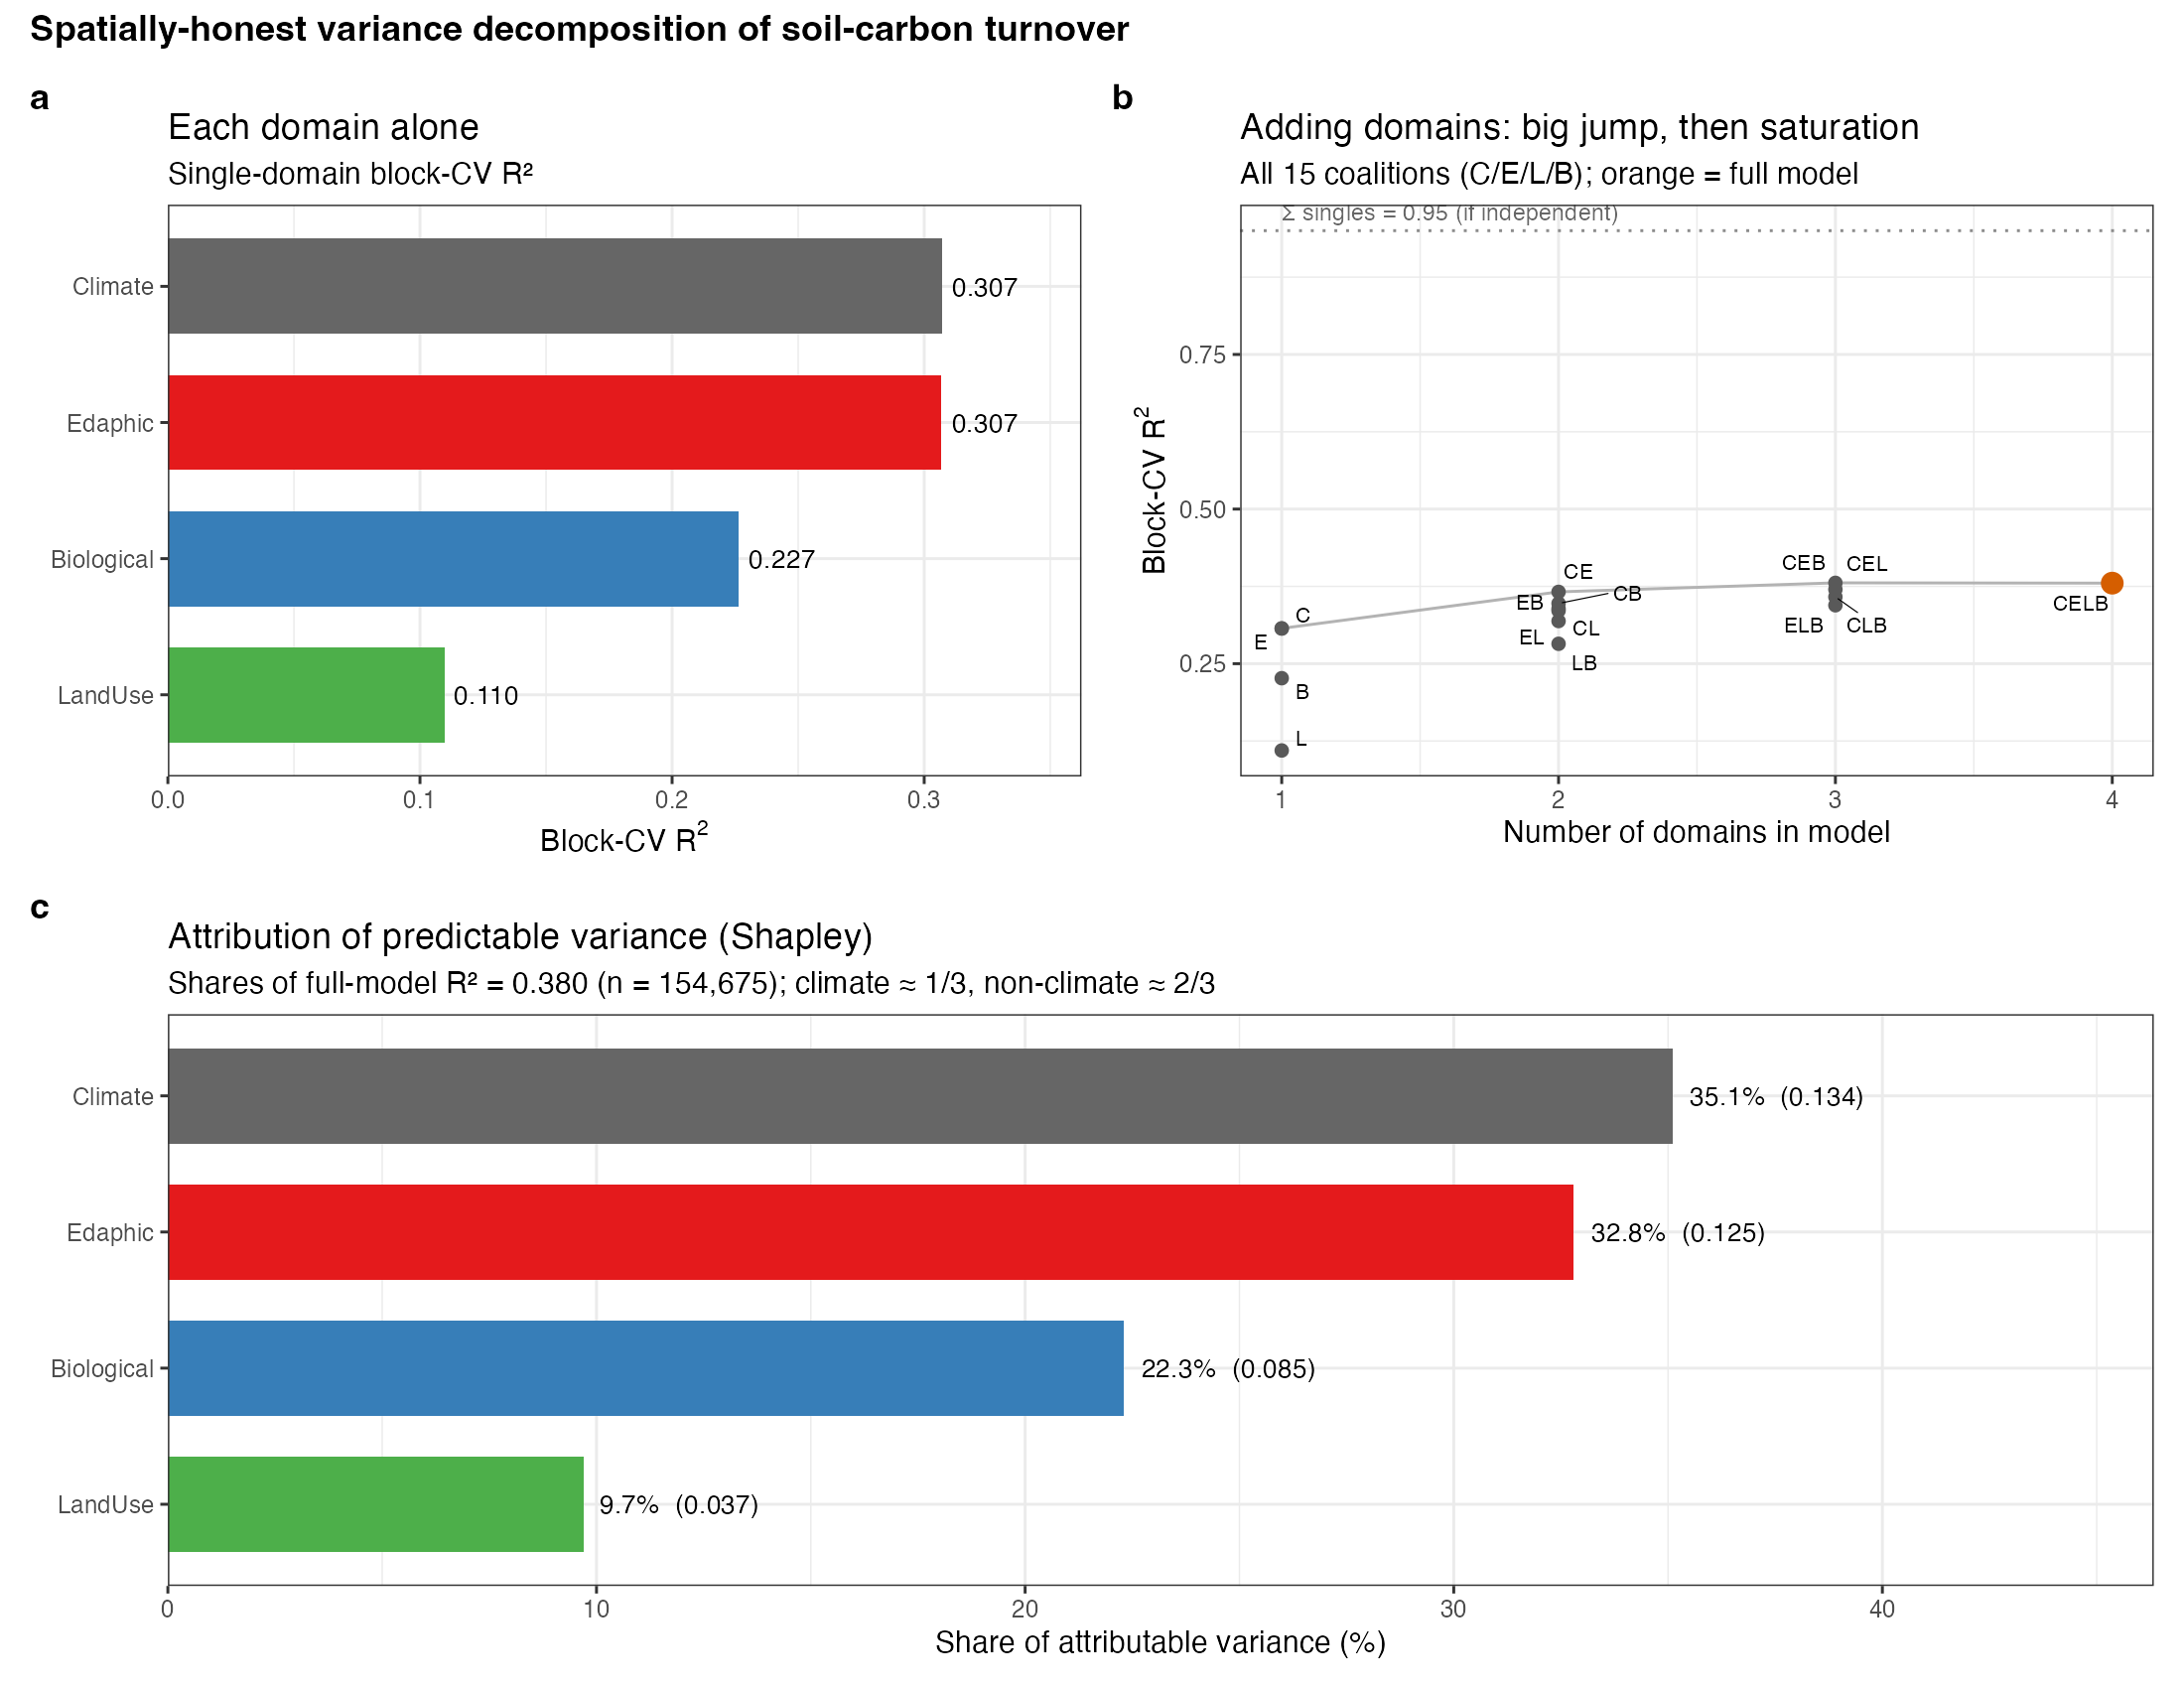
\includegraphics[width=0.96\textwidth]{../../plots/step_13c_commonality/13c_decomposition.png}
\caption{\textbf{Variance decomposition (Results).} Singles $\to$ build-up across
coalitions $\to$ Shapley shares. The build-up panel makes the overlap visible (the
full model sits far below the sum-of-singles line). \fpath{13c_results_figure.R}}
\end{figure}

\textbf{Is the residual organised? (Moran's $I$).} \textit{What Moran's $I$ does,
plainly:} it asks whether places close together have more similar values than chance
would give --- $I\approx0$ means spatially random, $I>0$ means clustered. The
beyond-climate residual gives $I=0.25$ ($p\ll0.001$) at 2\textdegree{}: modest, but
unambiguously non-random. The signal is structure, not noise. (Residual map and
Moran scatter: appendix.)

\subsection{Zonality map --- ``where?''}

We map the log-ratio of model predictions --- how much non-climate context bends
predicted turnover relative to a climate-only model --- at meso (2\textdegree)
scale. The \emph{symmetric} formulation (each domain relative to climate; no
abiotic-before-biology ordering) is the main figure, consistent with the
order-independent attribution. The abiotic panel is near-global over soil-bearing
land and shows a coherent geography: non-climate context \emph{lengthens} turnover
in the Amazon and Congo basins (deep, weathered, low-fertility clays that stabilise
carbon) and \emph{shortens} it across drylands (Sahel margins, central Asia,
Australia). This is the pattern that earns the word ``zonality.''

\textbf{Why meso scale --- the positive evidence.} We do not map at meso scale
merely because the native pixel is noisy; we map there because that is where the map
\emph{works}. We tested how well the beyond-climate map (full minus climate, both
out-of-sample) agrees with the observed residual as it is aggregated to coarser
blocks. Agreement roughly \emph{doubles} from the noisy native pixel
($R^2\approx0.11$) to $\approx0.22$ by 1--2\textdegree{} as point noise averages
out, then \emph{plateaus} across the 1--7\textdegree{} range. There is no single
privileged scale --- it is a plateau, not a peak --- and 2\textdegree{} sits
comfortably inside it (consistent with the $\sim$16~km variogram range and
$I=0.25$). A purely \emph{linear} skill proxy declines with scale and would have
missed this; the conclusion needs the nonlinear, map-faithful metric (appendix).

\begin{figure}[H]\centering
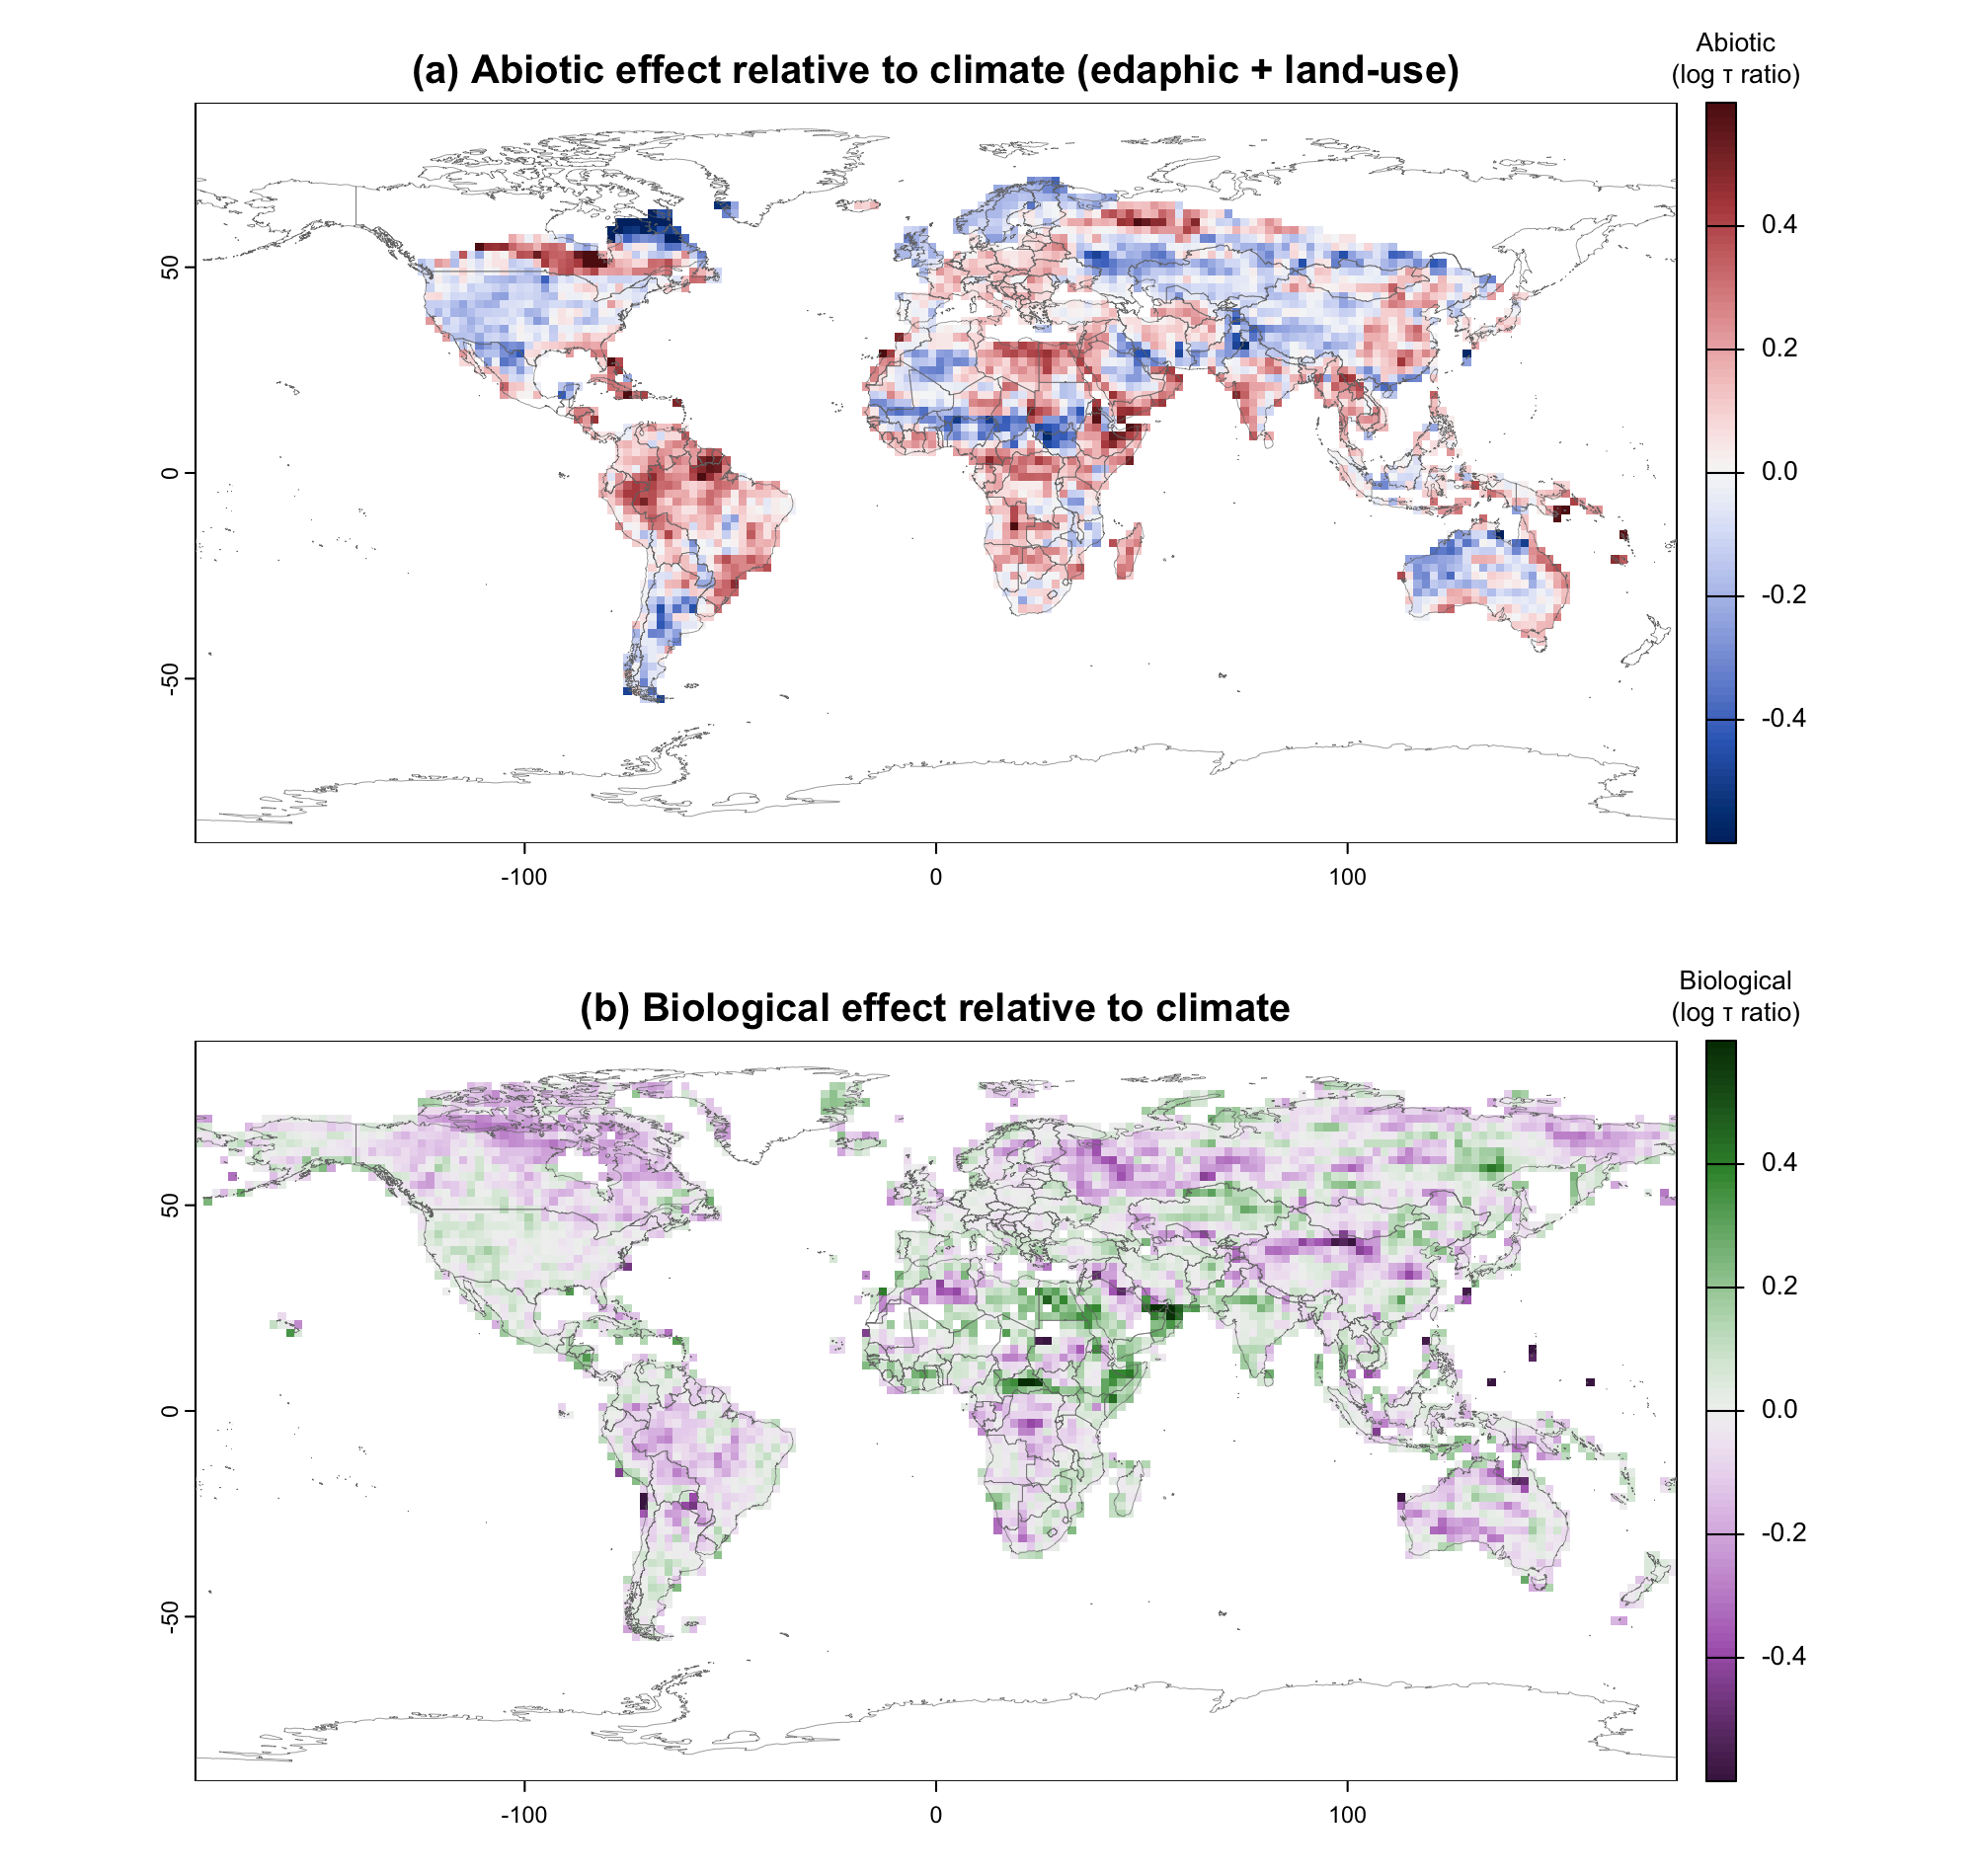
\includegraphics[width=0.82\textwidth]{../../plots/step_15b_zonality/zonality_map_dual_symmetric.png}
\caption{\textbf{Zonality map, symmetric (Results).} (a) Abiotic and (b) biological
modulation, each relative to climate. Red/green = longer turnover, blue/purple =
shorter. The abiotic panel doubles as the near-global headline. Nested formulation
and the abiotic-vs-biology scatter: appendix. \fpath{15b_zonality_map.R}}
\end{figure}

\subsection{Mechanism --- ``how?'' (ALE)}

Accumulated Local Effects give the marginal, functional response of turnover to each
predictor. \emph{(Now computed on the MAIN 6-layer biology model, consistent with
the attribution and the maps.)} The curves are clean and mechanistically sensible:
turnover increases with temperature seasonality, snow cover, and elevation;
decreases with sand fraction, bulk density, and soil temperature; and is humped in
pH. This is the layer that turns the attribution and the map into \emph{mechanism}
--- not just that edaphic matters and where, but \emph{how} each property acts.

\begin{figure}[H]\centering
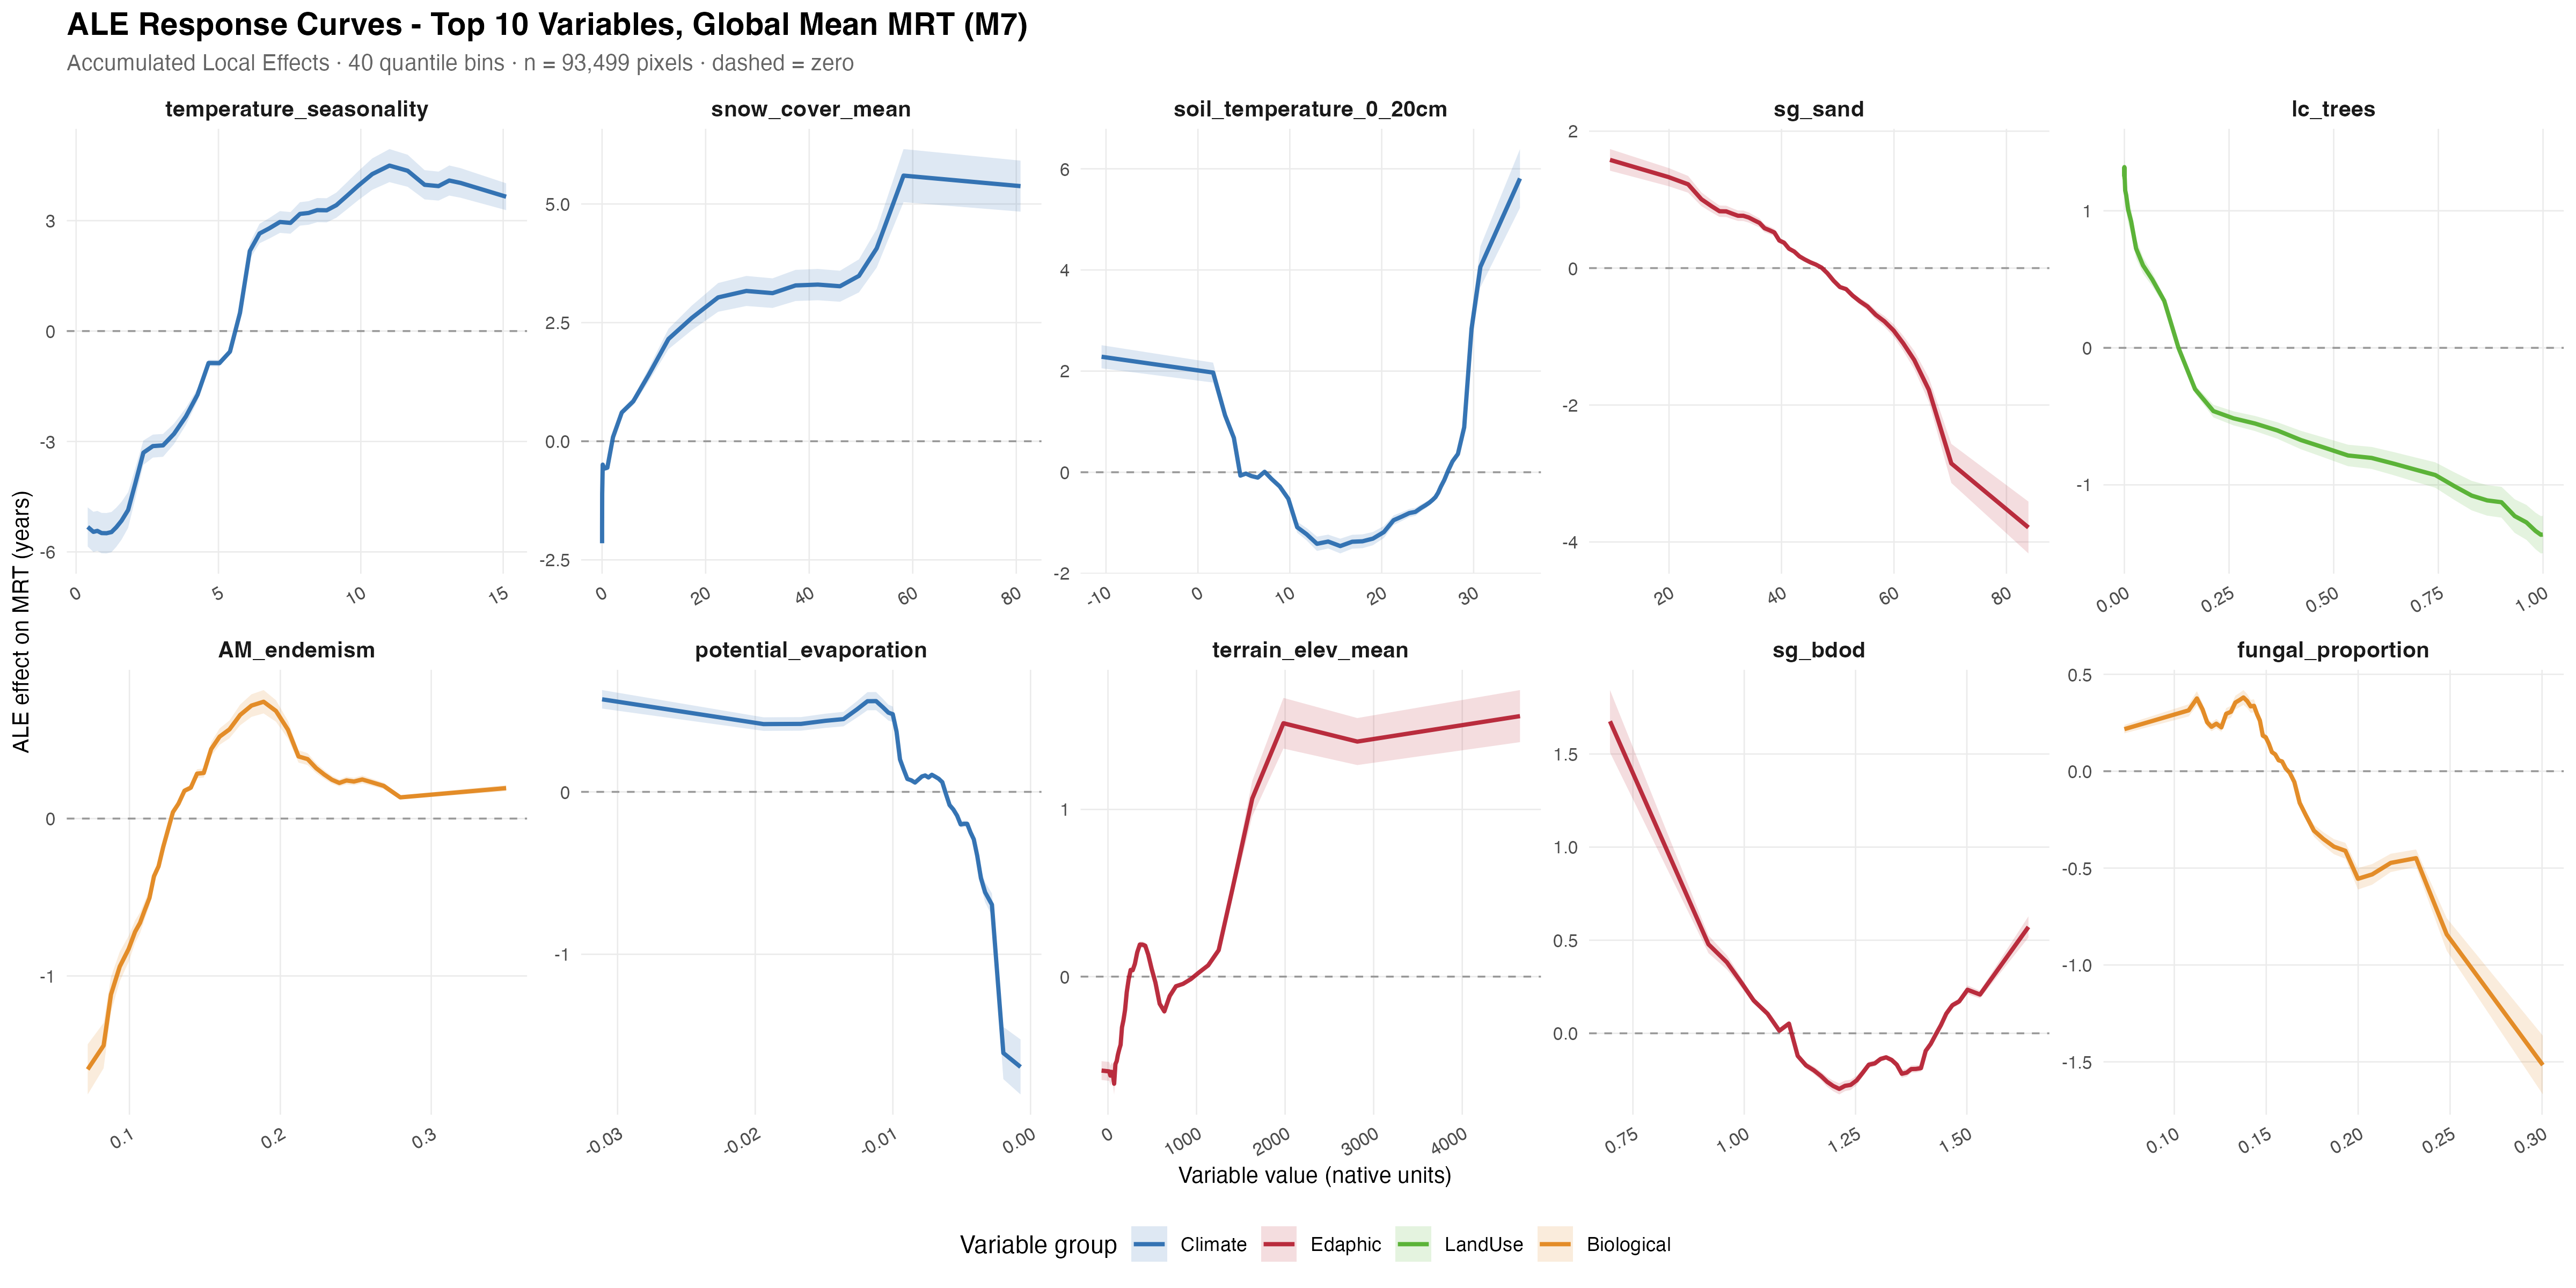
\includegraphics[width=0.96\textwidth]{../../plots/step_18_sensitivity/18D_ALE_top10_MRT.png}
\caption{\textbf{ALE response curves (Results).} Top-10 predictors, coloured by
domain; MAIN 6-layer biology model. \fpath{18_sensitivity_analysis.R}}
\end{figure}

\subsection{ESM contrast --- ``so what?''}

We compare the spatial \emph{structure} of turnover against six structurally
independent CMIP6 models. Absolute turnover times are not comparable across products
(depth, pool, and reference-period definitions differ), so we normalise each product
to its own global mean and compare structure --- a choice that pre-empts the
``apples to pears'' critique. We do not certify any model's absolute skill; we read
their spatial structure against the observational pattern. The result is sharp:
observations show a gentle zonality (polar turnover $\sim$2.5$\times$ tropical),
whereas individual ESMs amplify it far more --- a median of $\sim$9$\times$ across the
ensemble, up to $\sim$14$\times$ (CanESM5) --- while disagreeing among themselves across
more than an order of magnitude (0.6--14$\times$); one model (MPI) inverts the gradient.
The over-zonalization factor (ESM median vs observations) is $\sim$3.7$\times$. (On a
raster high-latitude $>$50\textdegree{}/tropical basis the ensemble mean gives a gentler
$\sim$5$\times$, factor $\sim$3.2$\times$ --- same direction, different aggregation.)

\begin{figure}[H]\centering
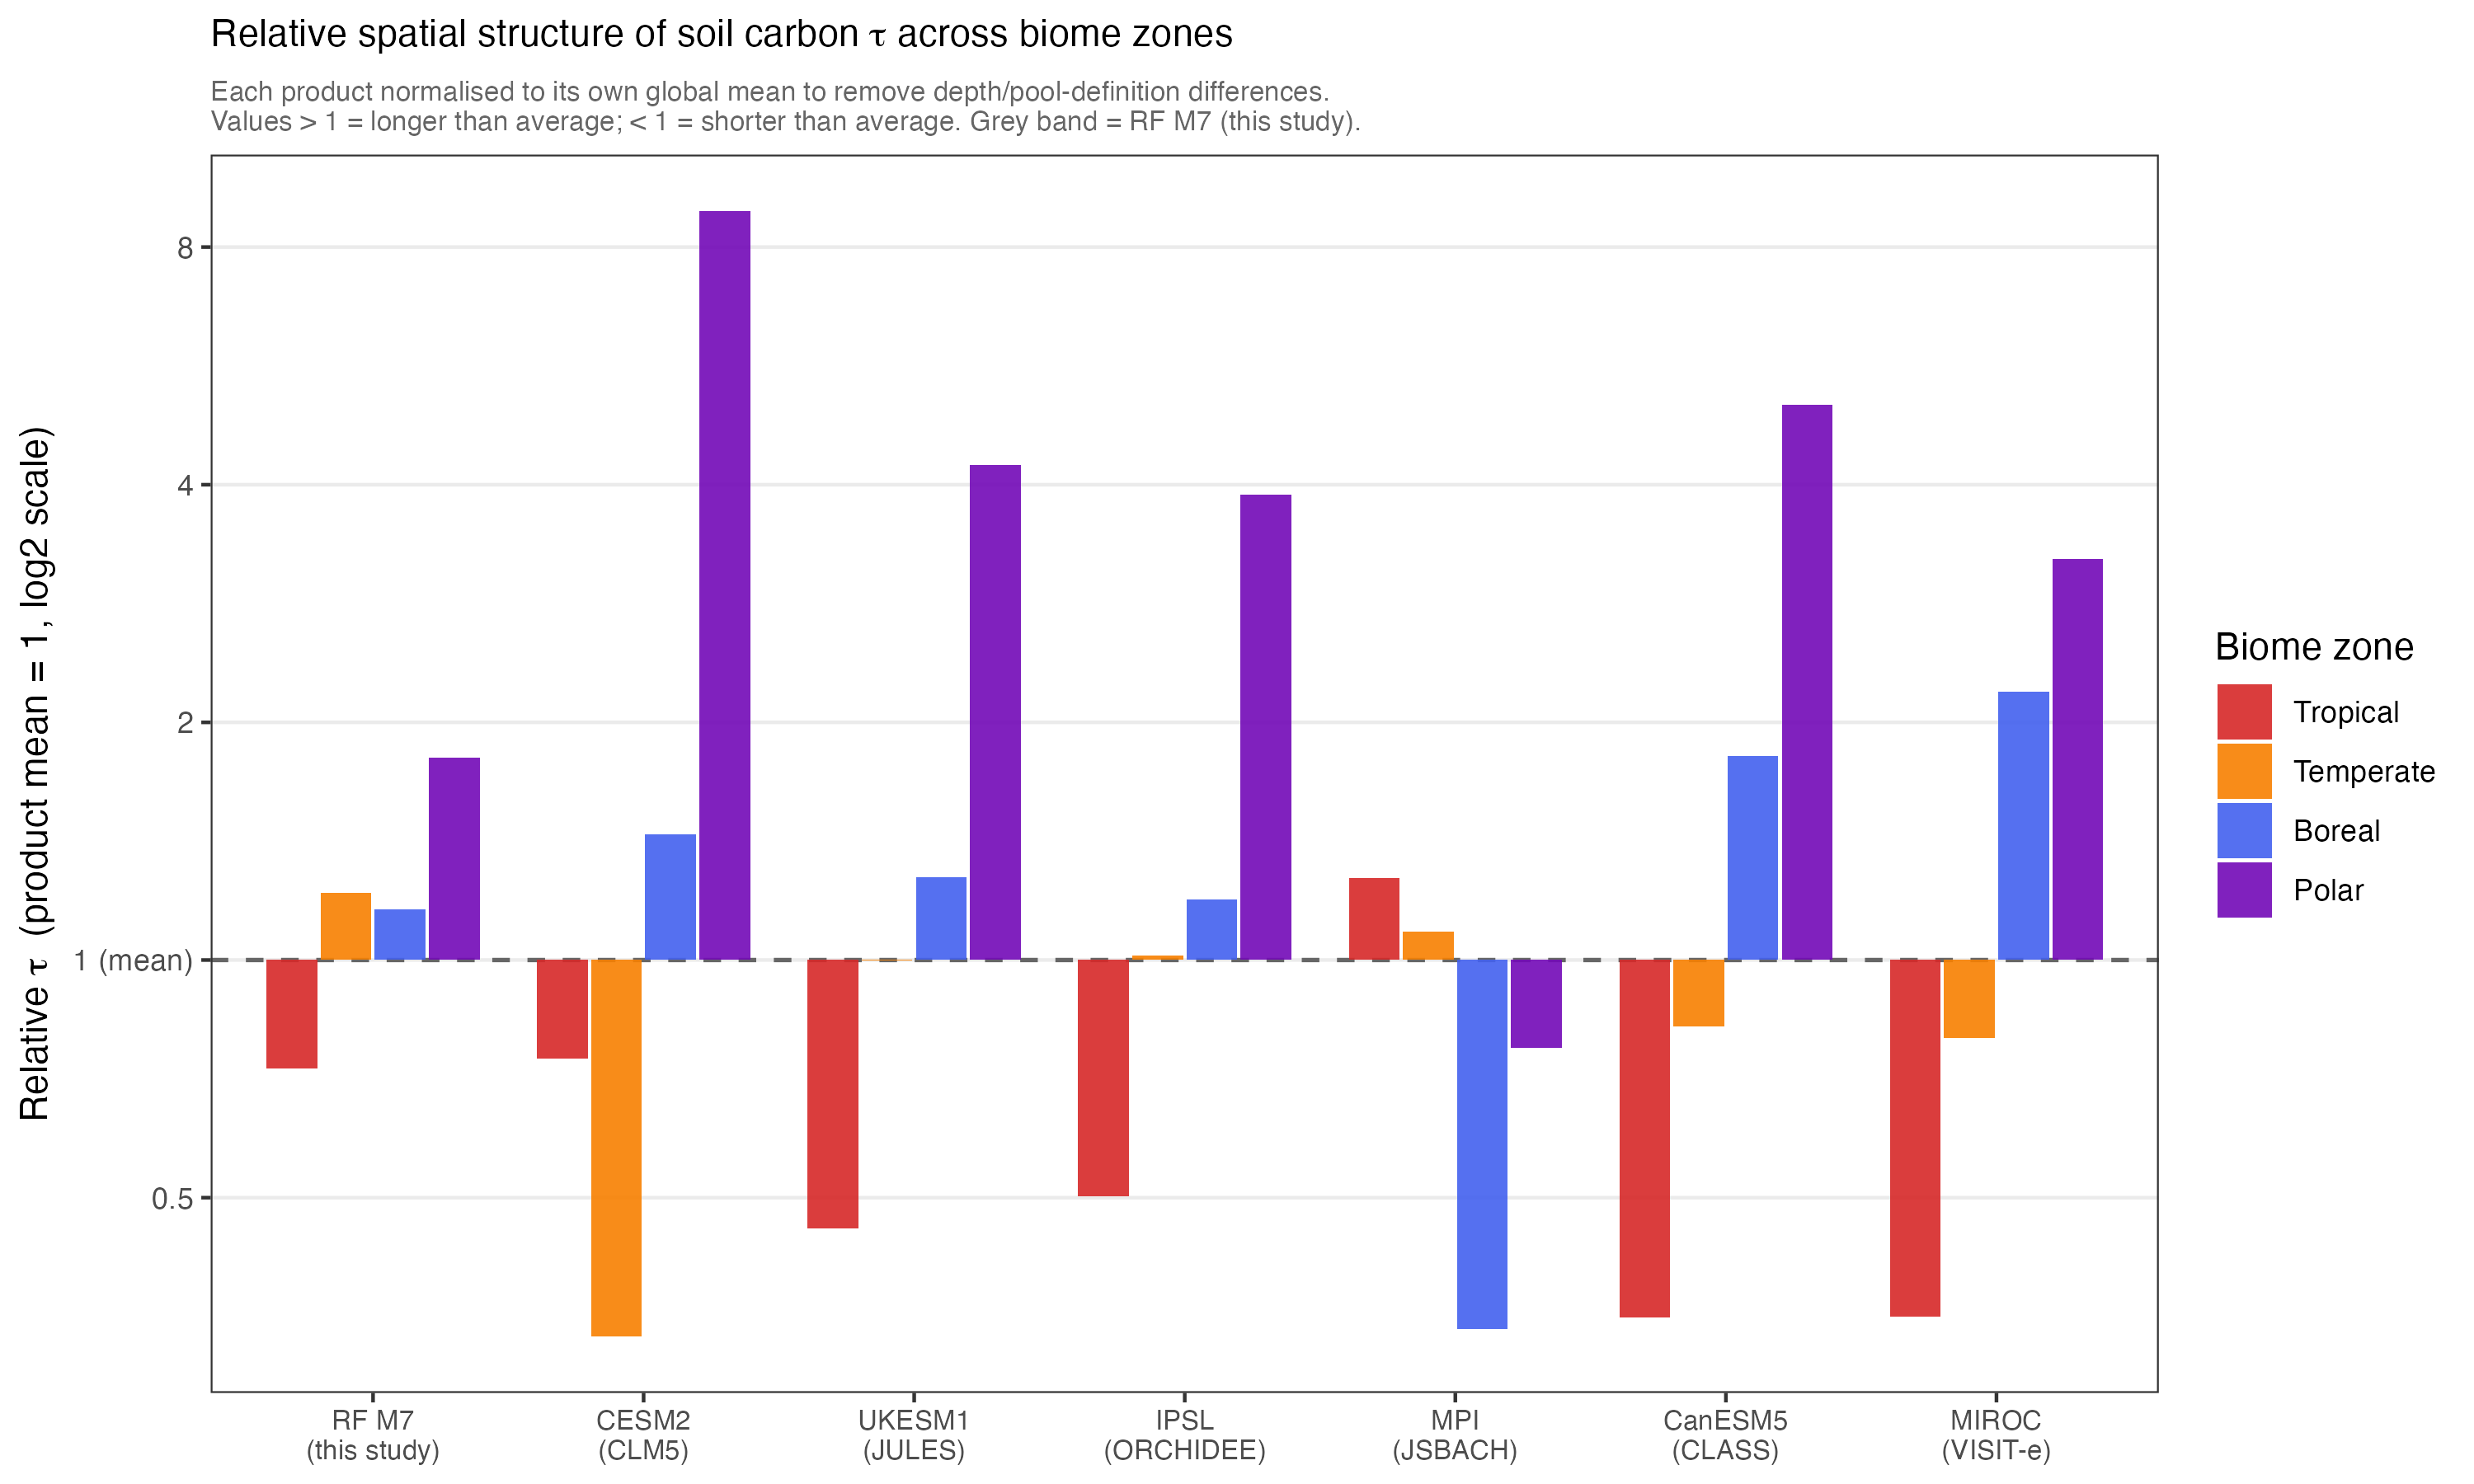
\includegraphics[width=0.96\textwidth]{../../plots/step_20/fig_biome_relative_tau.png}
\caption{\textbf{ESM structural comparison (Results).} Relative turnover by biome
zone, each product normalised to its own global mean. \fpath{20_CMIP_comparison.R};
amplification ratios \fpath{20b_zonal_amplification.R}}
\end{figure}

% =============================================================================
\section{Supporting analyses (robustness)}

These do not carry the argument; they make the modest signal trustworthy. Each is a
numbered, repeatable script. Figures are in the appendix.

\textbf{Spatial block cross-validation.} All skill is estimated by holding out whole
2\textdegree{} blocks, so reported $R^2$ is out-of-region generalisation, not
interpolation between near-neighbours.

\textbf{Noise floor and mapping scale.} The residual variogram has nugget/sill
$\sim$0.56 and range $\sim$16~km: roughly two thirds of the beyond-climate residual
is unstructured noise, structured only at short range. The RF mapping-skill curve
(above) shows the complementary positive result --- aggregating to meso scale
roughly doubles map--truth agreement and then plateaus. Together they justify mapping
at meso scale and never showing native-pixel texture.

\textbf{Provenance control.} Only 2.4\% of the residual variance lies between the 44
source databases; removing each source's mean barely changes the coarse organisation
or covariate skill. The signal is ecological, not a laboratory/compilation artifact
(conservative, since source is confounded with geography).

\textbf{Biological parsimony.} The biological signal is multidimensional, but the
three Barcel\'o root-colonisation layers are statistically inert ($+0.001$ unique
$R^2$) while capping coverage. Dropping them lifts the biological footprint from 61\%
to 96\% of sampled rows with no loss of skill; the full nine-layer set is kept as a
sensitivity case.

\textbf{Block-size invariance.} Re-running the decomposition with 1\textdegree{} and
5\textdegree{} blocks (now at the production 500 trees) moves each Shapley share by
at most \textbf{2.5 percentage points}, even though absolute $R^2$ declines with
block size (0.40 / 0.38 / 0.34 at 1 / 2 / 5\textdegree) --- attribution is robust to
the scale choice.

\textbf{Spatial correlation of the two axes.} Abiotic and biological modulation
co-vary when each is taken over climate ($r\approx0.4$--$0.5$) but are orthogonal once
biology is taken conditional on the abiotic model ($r\approx0$). This is the
``correlated, not redundant'' result expressed spatially (appendix scatter,
K\"oppen-coloured).

% =============================================================================
\section{Key numbers}

\begin{table}[H]\centering\small
\begin{tabular}{ll}
\toprule
Quantity & Value \\
\midrule
Full-model block-CV $R^2$ & 0.38 (climate alone 0.31; beyond-climate $\sim$7~pp) \\
Shapley shares (C/E/B/L) & 35 / 33 / 22 / 10 \% \\
Single-domain $R^2$ & C 0.31 $\approx$ E 0.31 $>$ B 0.23 $\gg$ L 0.11 \\
Overlap ($\Sigma$ singles $-$ full) & 0.57 (correlated, not redundant) \\
Spatial organisation (Moran's $I$) & 0.25 ($p\ll0.001$) at 2\textdegree \\
Noise floor (nugget/sill; range) & 0.56; $\sim$16~km \\
Map skill vs scale (RF) & native $R^2\approx0.11 \to \approx0.22$ at 1--2\textdegree, plateau 1--7\textdegree \\
Between-source variance share & 2.4\% (ecological, not provenance) \\
Block-size invariance (500 trees) & shares move $\le$2.5~pp over 1--5\textdegree \\
Biological coverage (MAIN set) & 96\% of rows (vs 61\% with Barcel\'o) \\
Over-zonalization (ESM vs obs) & polar/tropical 2.5$\times$ (obs) vs ESM median $\sim$9$\times$ (0.6--14); factor $\sim$3.7$\times$ \\
\bottomrule
\end{tabular}
\end{table}

% =============================================================================
\section{Figure plan}

\begin{table}[H]\centering\small
\begin{tabular}{lll}
\toprule
Figure & Destination & Comment \\
\midrule
Variance decomposition & Results & how much + the overlap keystone \\
Zonality map (symmetric) & Results & where; abiotic panel = near-global headline \\
ALE response curves (6-layer) & Results & how each driver acts (mechanism) \\
ESM biome-relative & Results & so what; structural over-zonalization \\
RF mapping skill vs scale & Appendix & \textbf{new}; meso-scale justification (plateau) \\
Scale / noise-floor & Appendix & two-thirds noise; short-range structure \\
Tier-1 residual map + Moran & Appendix & organisation is real, not noise \\
Block-size sensitivity (500 tr.) & Appendix/Methods & justifies 2\textdegree; $\le$2.5~pp \\
Biological parsimony & Appendix & why drop Barcel\'o; keep 9 as sensitivity \\
Nested map + abiotic/biology scatter & Appendix & order-dependence; correlated-not-redundant \\
Relative latitude heatmap & Appendix/SI & continuous-latitude ESM structure \\
Absolute latitudinal profile & Appendix & the resolved-tension side-arc \\
Sampling coverage & Methods/Data & where/when sampled \\
\midrule
\textit{Dropped (obsolete)} & --- & step-17 M1--M7 maps, all-models comparison, \\
 & & latitude histogram; step-20 absolute heatmap; \\
 & & standalone linear skill proxy (folded into RF figure) \\
\bottomrule
\end{tabular}
\end{table}

% =============================================================================
\section{A note on the biology axis (literature to expand)}

The claim that soil biology forms a \emph{distinct second axis} of turnover --- the
most novel and the most contestable part of the story --- is currently
under-supported by citations. Before it lands in the manuscript it needs an expanded
literature scaffold: the mycorrhizal-type / carbon-persistence literature (AM vs EcM
economies), the SPUN richness/endemism layers and what they do and do not measure,
and the debate over whether microbial community structure carries independent
predictive information about carbon turnover beyond what climate and soil chemistry
already encode. Treat this as a writing task, not an analysis task.

% =============================================================================
\section{Two deliberate narrative devices}

\textbf{Own the incomparability.} In the ESM section we state up front that absolute
turnover is not comparable across products, and therefore compare only normalised
spatial structure. Declaring the limitation first, and controlling for it, converts a
potential ``apples to pears'' objection into a deliberate design choice.

\textbf{Resolved-tension side-arc (Discussion).} We briefly raise the
absolute-magnitude caveat (with the absolute latitudinal profile in the appendix) and
then resolve it via the structural comparison. A small arc for robustness, signalling
we considered and dismissed the obvious objection; not central.

% =============================================================================
\section{Status and next steps}

\textbf{Settled.} Shapley-primary lead; tool-first framing; symmetric map as the
Results centerpiece with the nested version and the scatter in the appendix; the
abiotic-vs-biology correlation reported briefly in the Discussion; the ESM section
reframed as structural comparison; step-17 demoted, step-18 kept, step-20's absolute
profile moved to the appendix side-arc.

\textbf{Analyses --- all landed.} (1) RF mapping-skill curve confirms the meso-scale
choice (plateau across 1--7\textdegree). (2) ALE and prediction maps regenerated on
the MAIN 6-layer biology, consistent with the attribution. (3) Block-size sweep
refreshed at 500 trees ($\le$2.5~pp invariance). (4) ESM comparison refreshed against
the 6-layer M7 map. Nothing analytical is outstanding.

\textbf{Open (cosmetic).} A minimum-fill coverage threshold for the meso maps; an
optional per-pixel Shapley map as the order-free gold standard (needs a step-14
extension).

\textbf{Next.} The prose pass: draft \fpath{manuscript.tex} section by section
against this outline and the reconciliation memo --- honouring the register and
framing notes above (pedological through-line; no self-advertising language; expanded
biology literature; Shapley and Moran explained for the reader).

% =============================================================================
\clearpage
\section{Appendix figures}

\textit{Collected here as they would appear at the end of the manuscript
(Appendix / Supplementary Information / Methods-Data). Main-text figures are inline
above.}

\begin{figure}[H]\centering
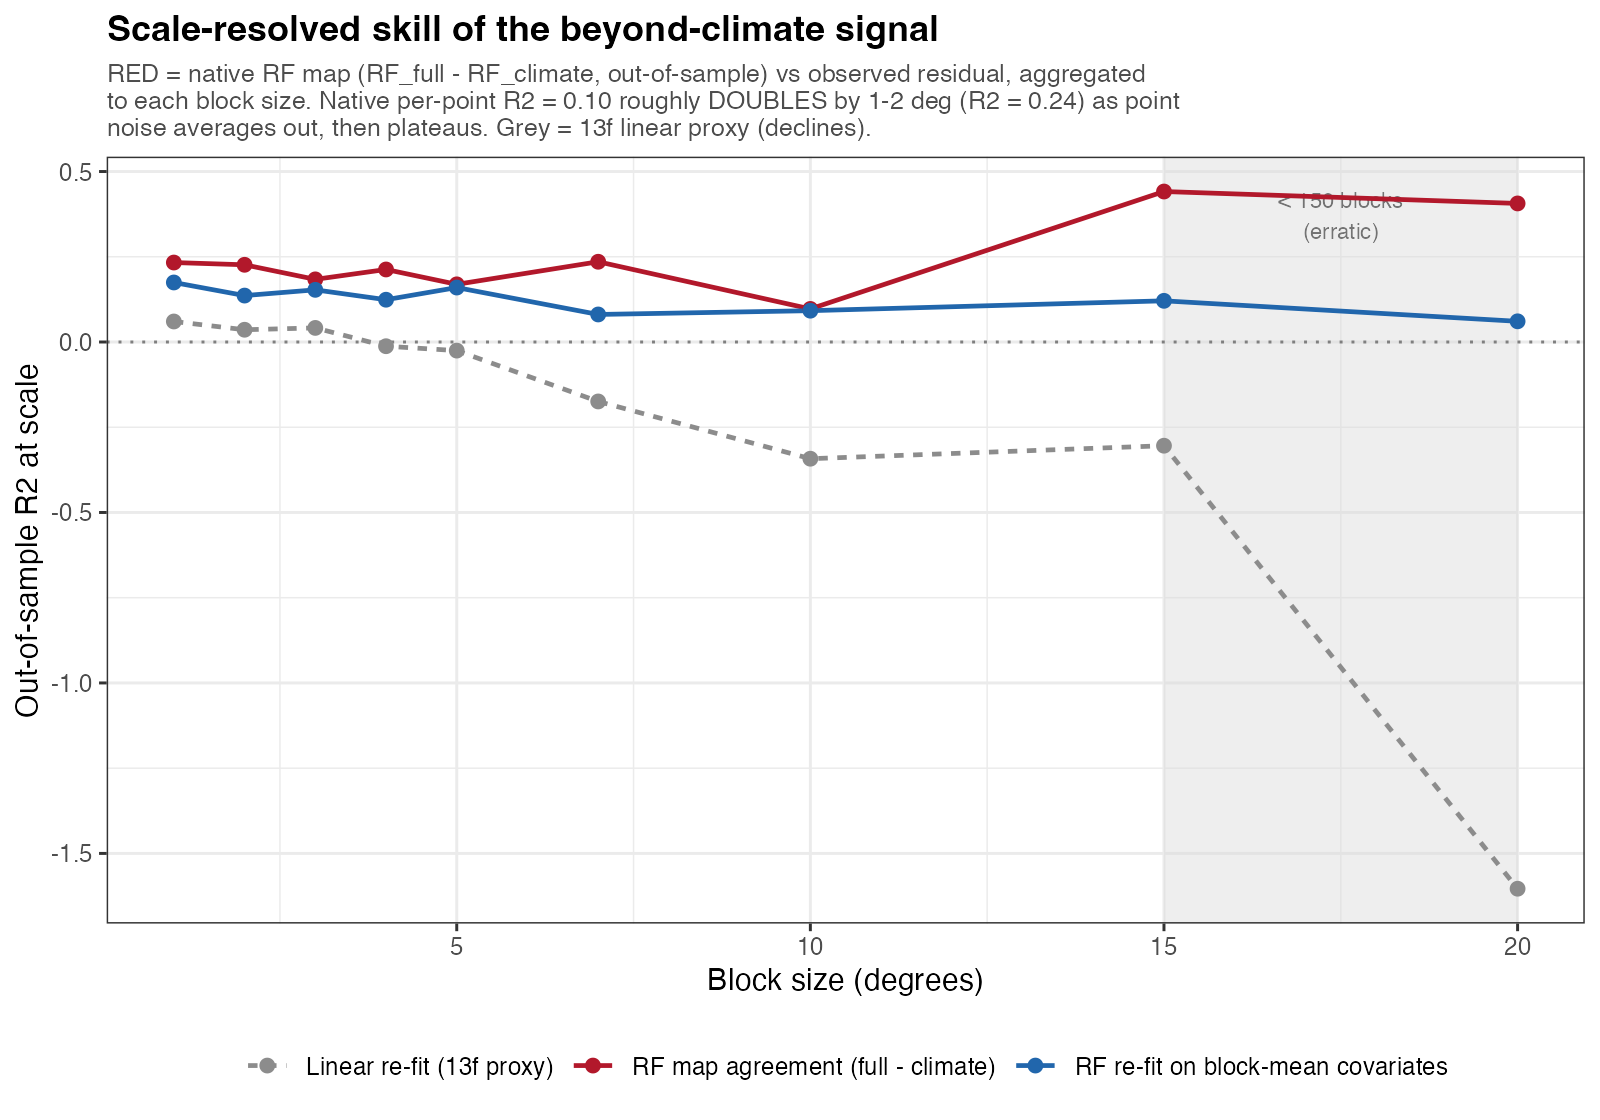
\includegraphics[width=0.85\textwidth]{../../plots/appendix/scale_rf_mapping_skill.png}
\caption{\textbf{[Appendix] RF mapping skill vs scale (new).} Agreement of the native
beyond-climate map (RF full $-$ RF climate, out-of-sample) with the observed residual,
aggregated to each block size. Native $R^2\approx0.11$ roughly doubles by
1--2\textdegree{} and plateaus across 1--7\textdegree; the linear proxy (grey)
declines. Coarse scales ($>$10\textdegree, shaded) have $<$150 blocks and are erratic.
This is the positive justification for meso-scale mapping. \fpath{13i_rf_scale_skill.R}}
\end{figure}

\begin{figure}[H]\centering
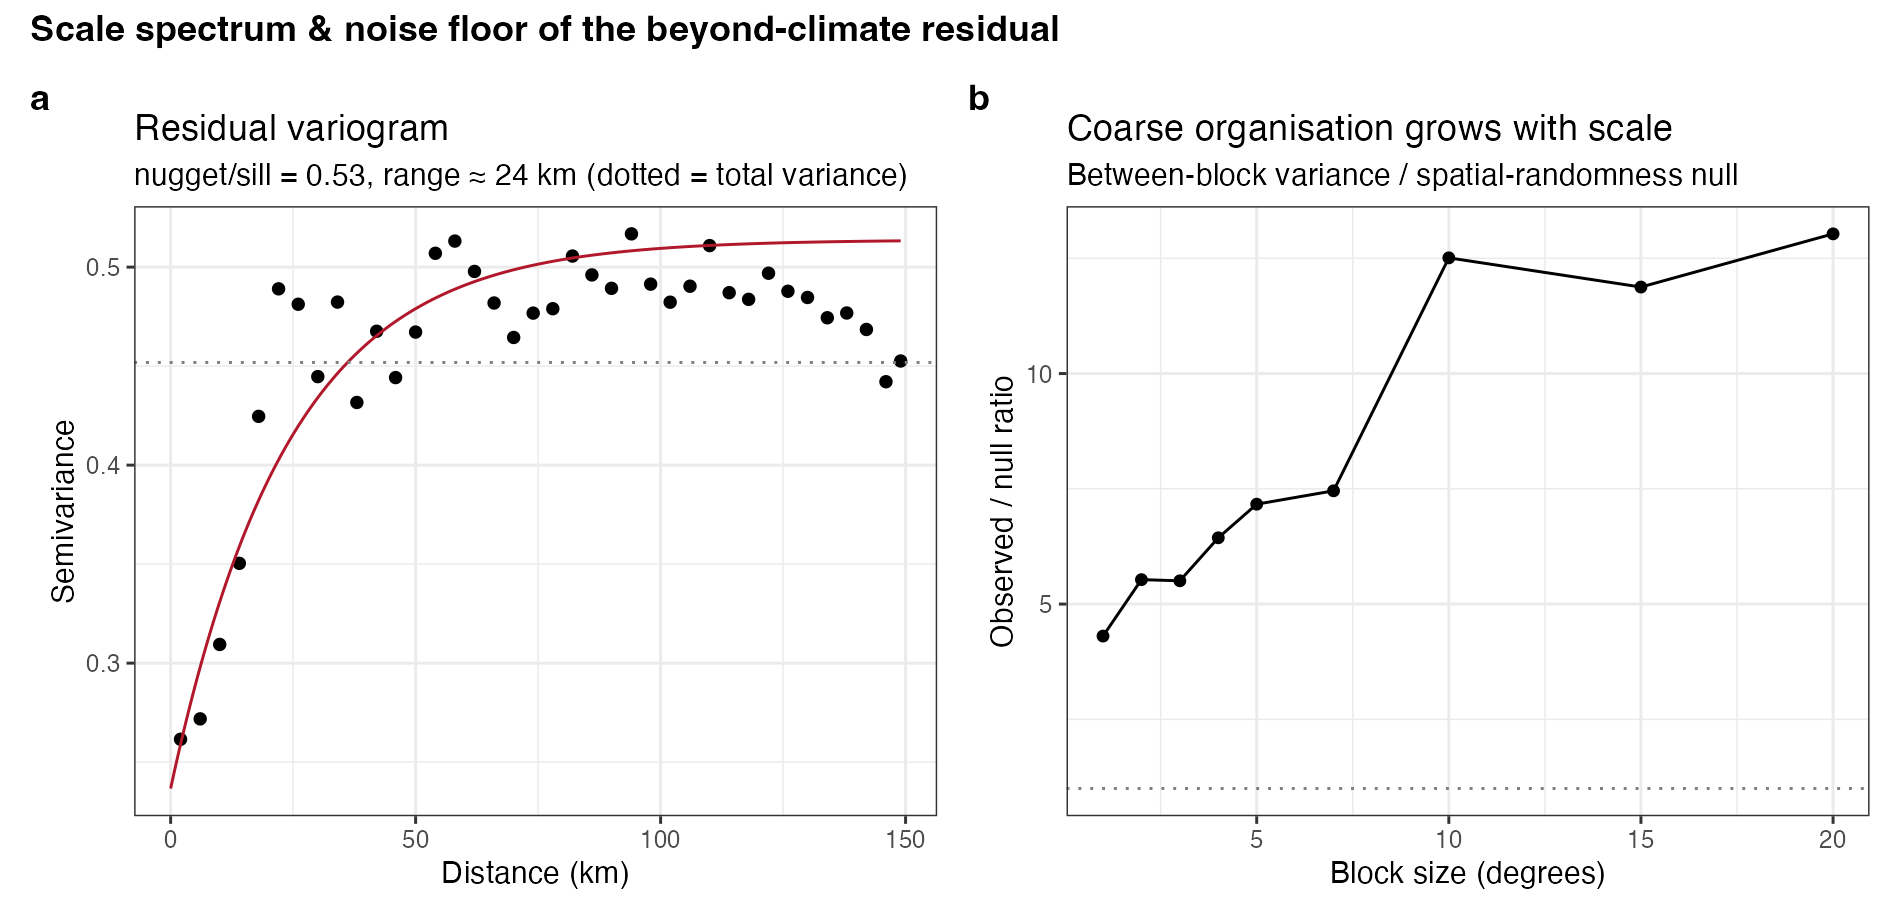
\includegraphics[width=0.95\textwidth]{../../plots/appendix/scale_noisefloor.png}
\caption{\textbf{[Appendix] Scale spectrum and noise floor.} (a) Residual variogram
(nugget/sill $\approx0.56$, range $\approx16$~km). (b) Coarse organisation grows with
block size. \fpath{13f_scale_noisefloor.R}}
\end{figure}

\begin{figure}[H]\centering
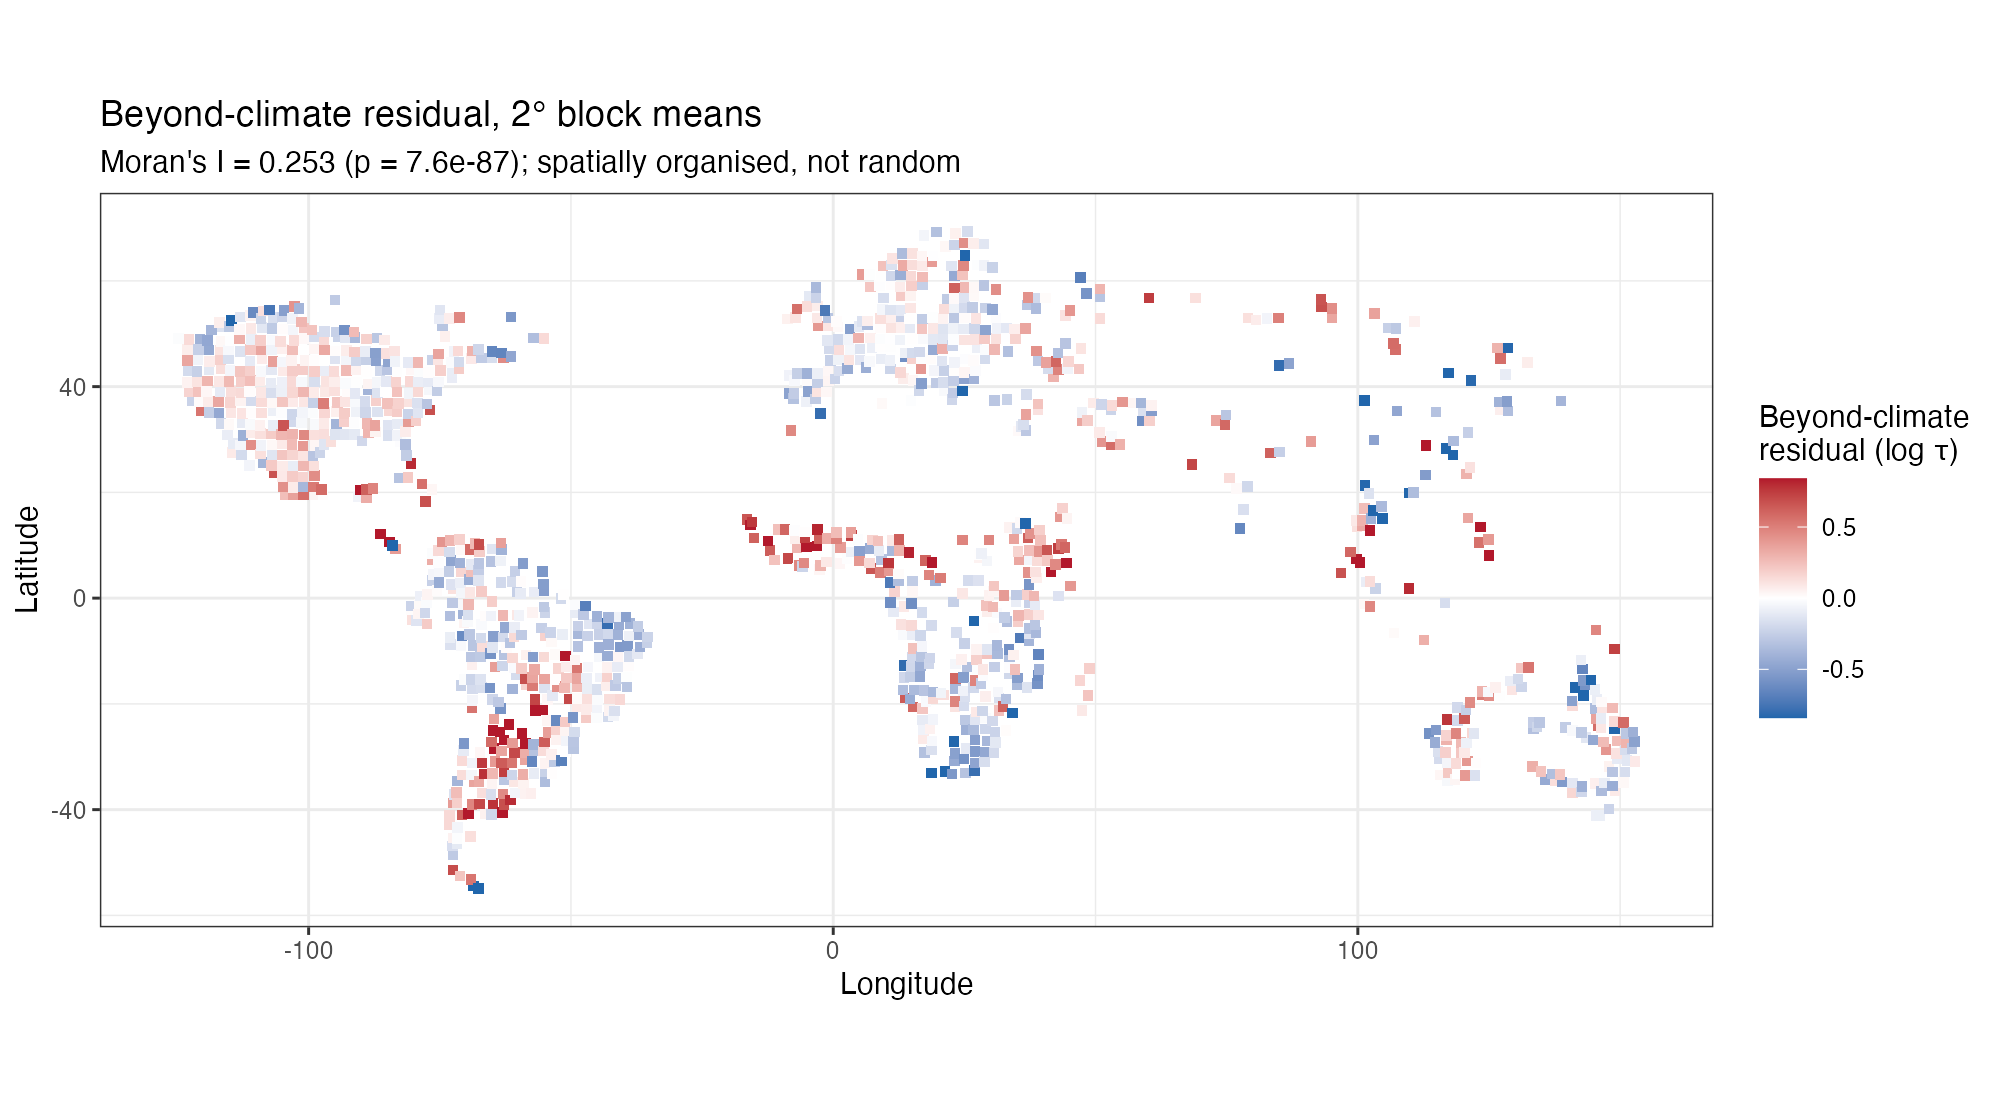
\includegraphics[width=0.49\textwidth]{../../plots/step_13c_commonality/13e_block_residual_map.png}
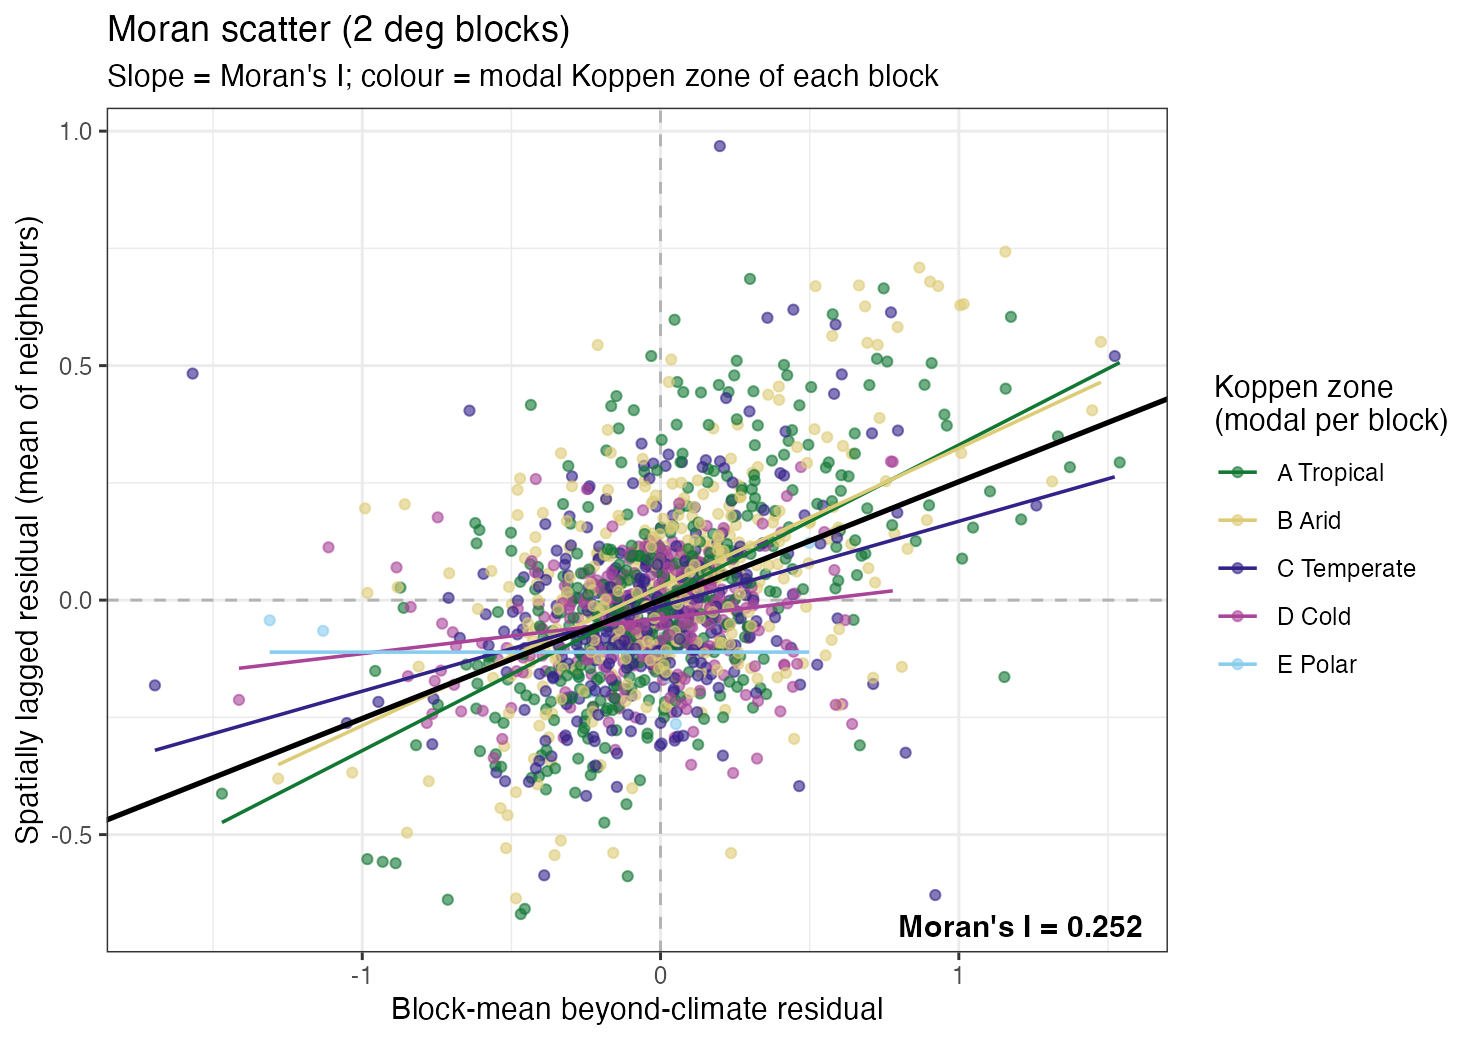
\includegraphics[width=0.49\textwidth]{../../plots/step_13c_commonality/13e_moran_scatter.png}
\caption{\textbf{[Appendix] Tier-1 spatial organisation.} Left: block-mean
beyond-climate residual map. Right: Moran scatter ($I=0.25$, $p\ll0.001$). The
residual is spatially organised, not noise. \fpath{13e_tier1_morans_i.R}}
\end{figure}

\begin{figure}[H]\centering
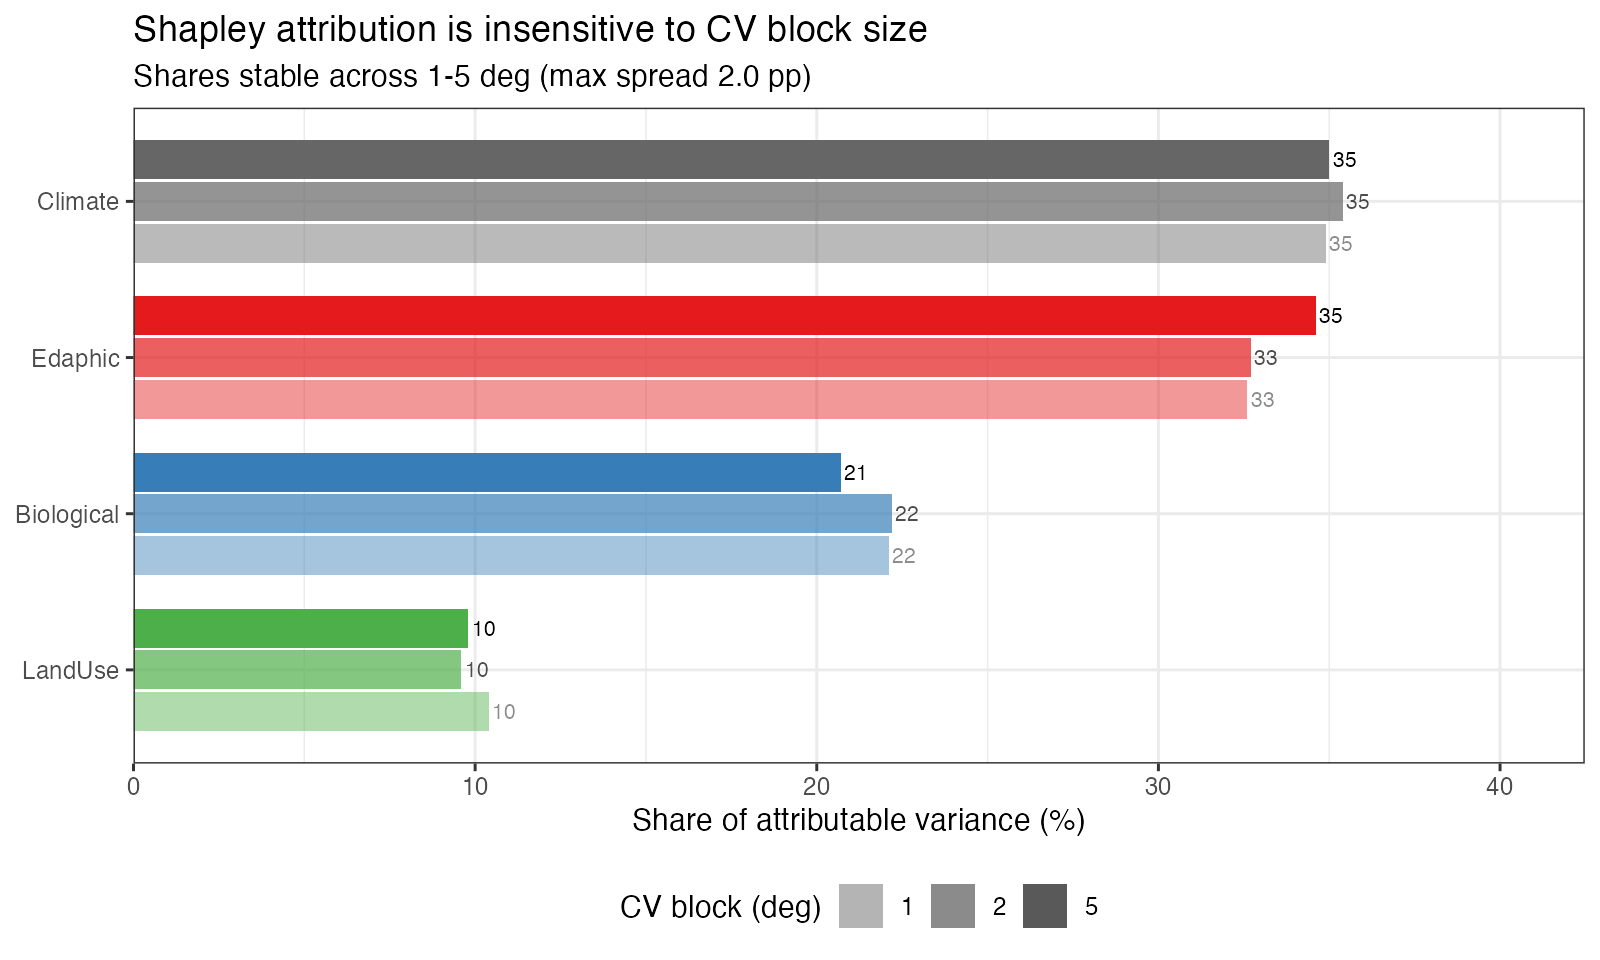
\includegraphics[width=0.80\textwidth]{../../plots/step_13c_commonality/13h_blocksize_shapley.png}
\caption{\textbf{[Appendix/Methods] Block-size invariance (500 trees).} Shapley shares
across 1/2/5\textdegree{} CV blocks; max spread $\le$2.5~pp despite the decline in
absolute $R^2$. \fpath{13h_blocksize_sensitivity.R}}
\end{figure}

\clearpage
\begin{figure}[H]\centering
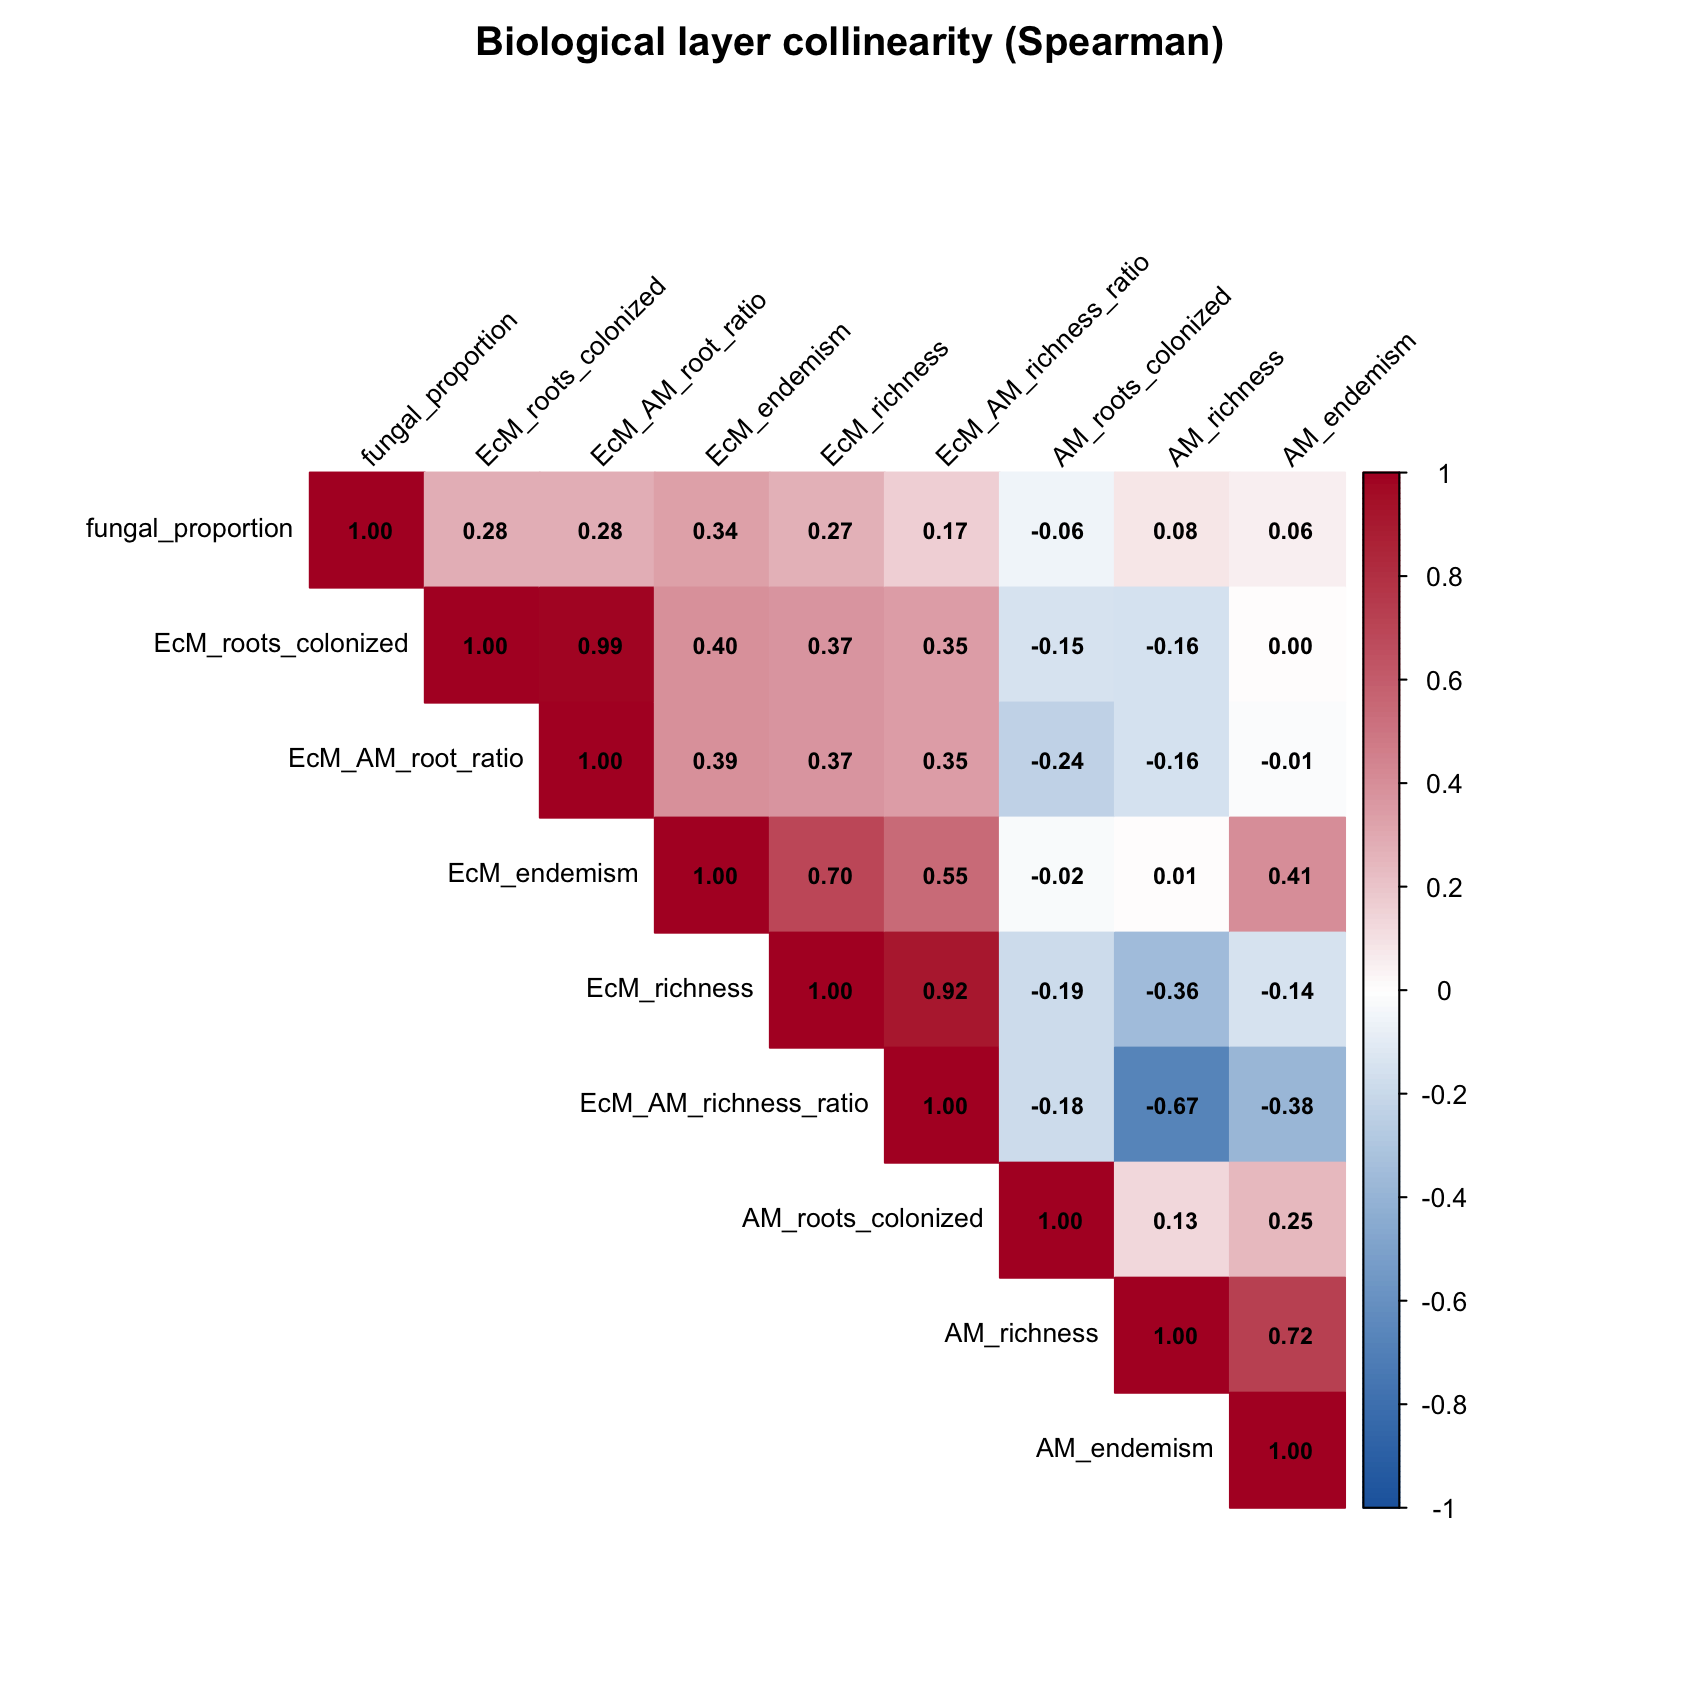
\includegraphics[width=0.49\textwidth]{../../plots/appendix/biological_collinearity.png}
\includegraphics[width=0.49\textwidth]{../../plots/appendix/biological_single_layer_skill.png}
\caption{\textbf{[Appendix] Biological parsimony.} Left: collinearity among the nine
biological layers. Right: single-layer skill vs coverage. Justifies dropping the three
Barcel\'o layers (inert, coverage-capping) for the MAIN 6-layer set.
\fpath{13d_biological_parsimony.R}}
\end{figure}

\begin{figure}[H]\centering
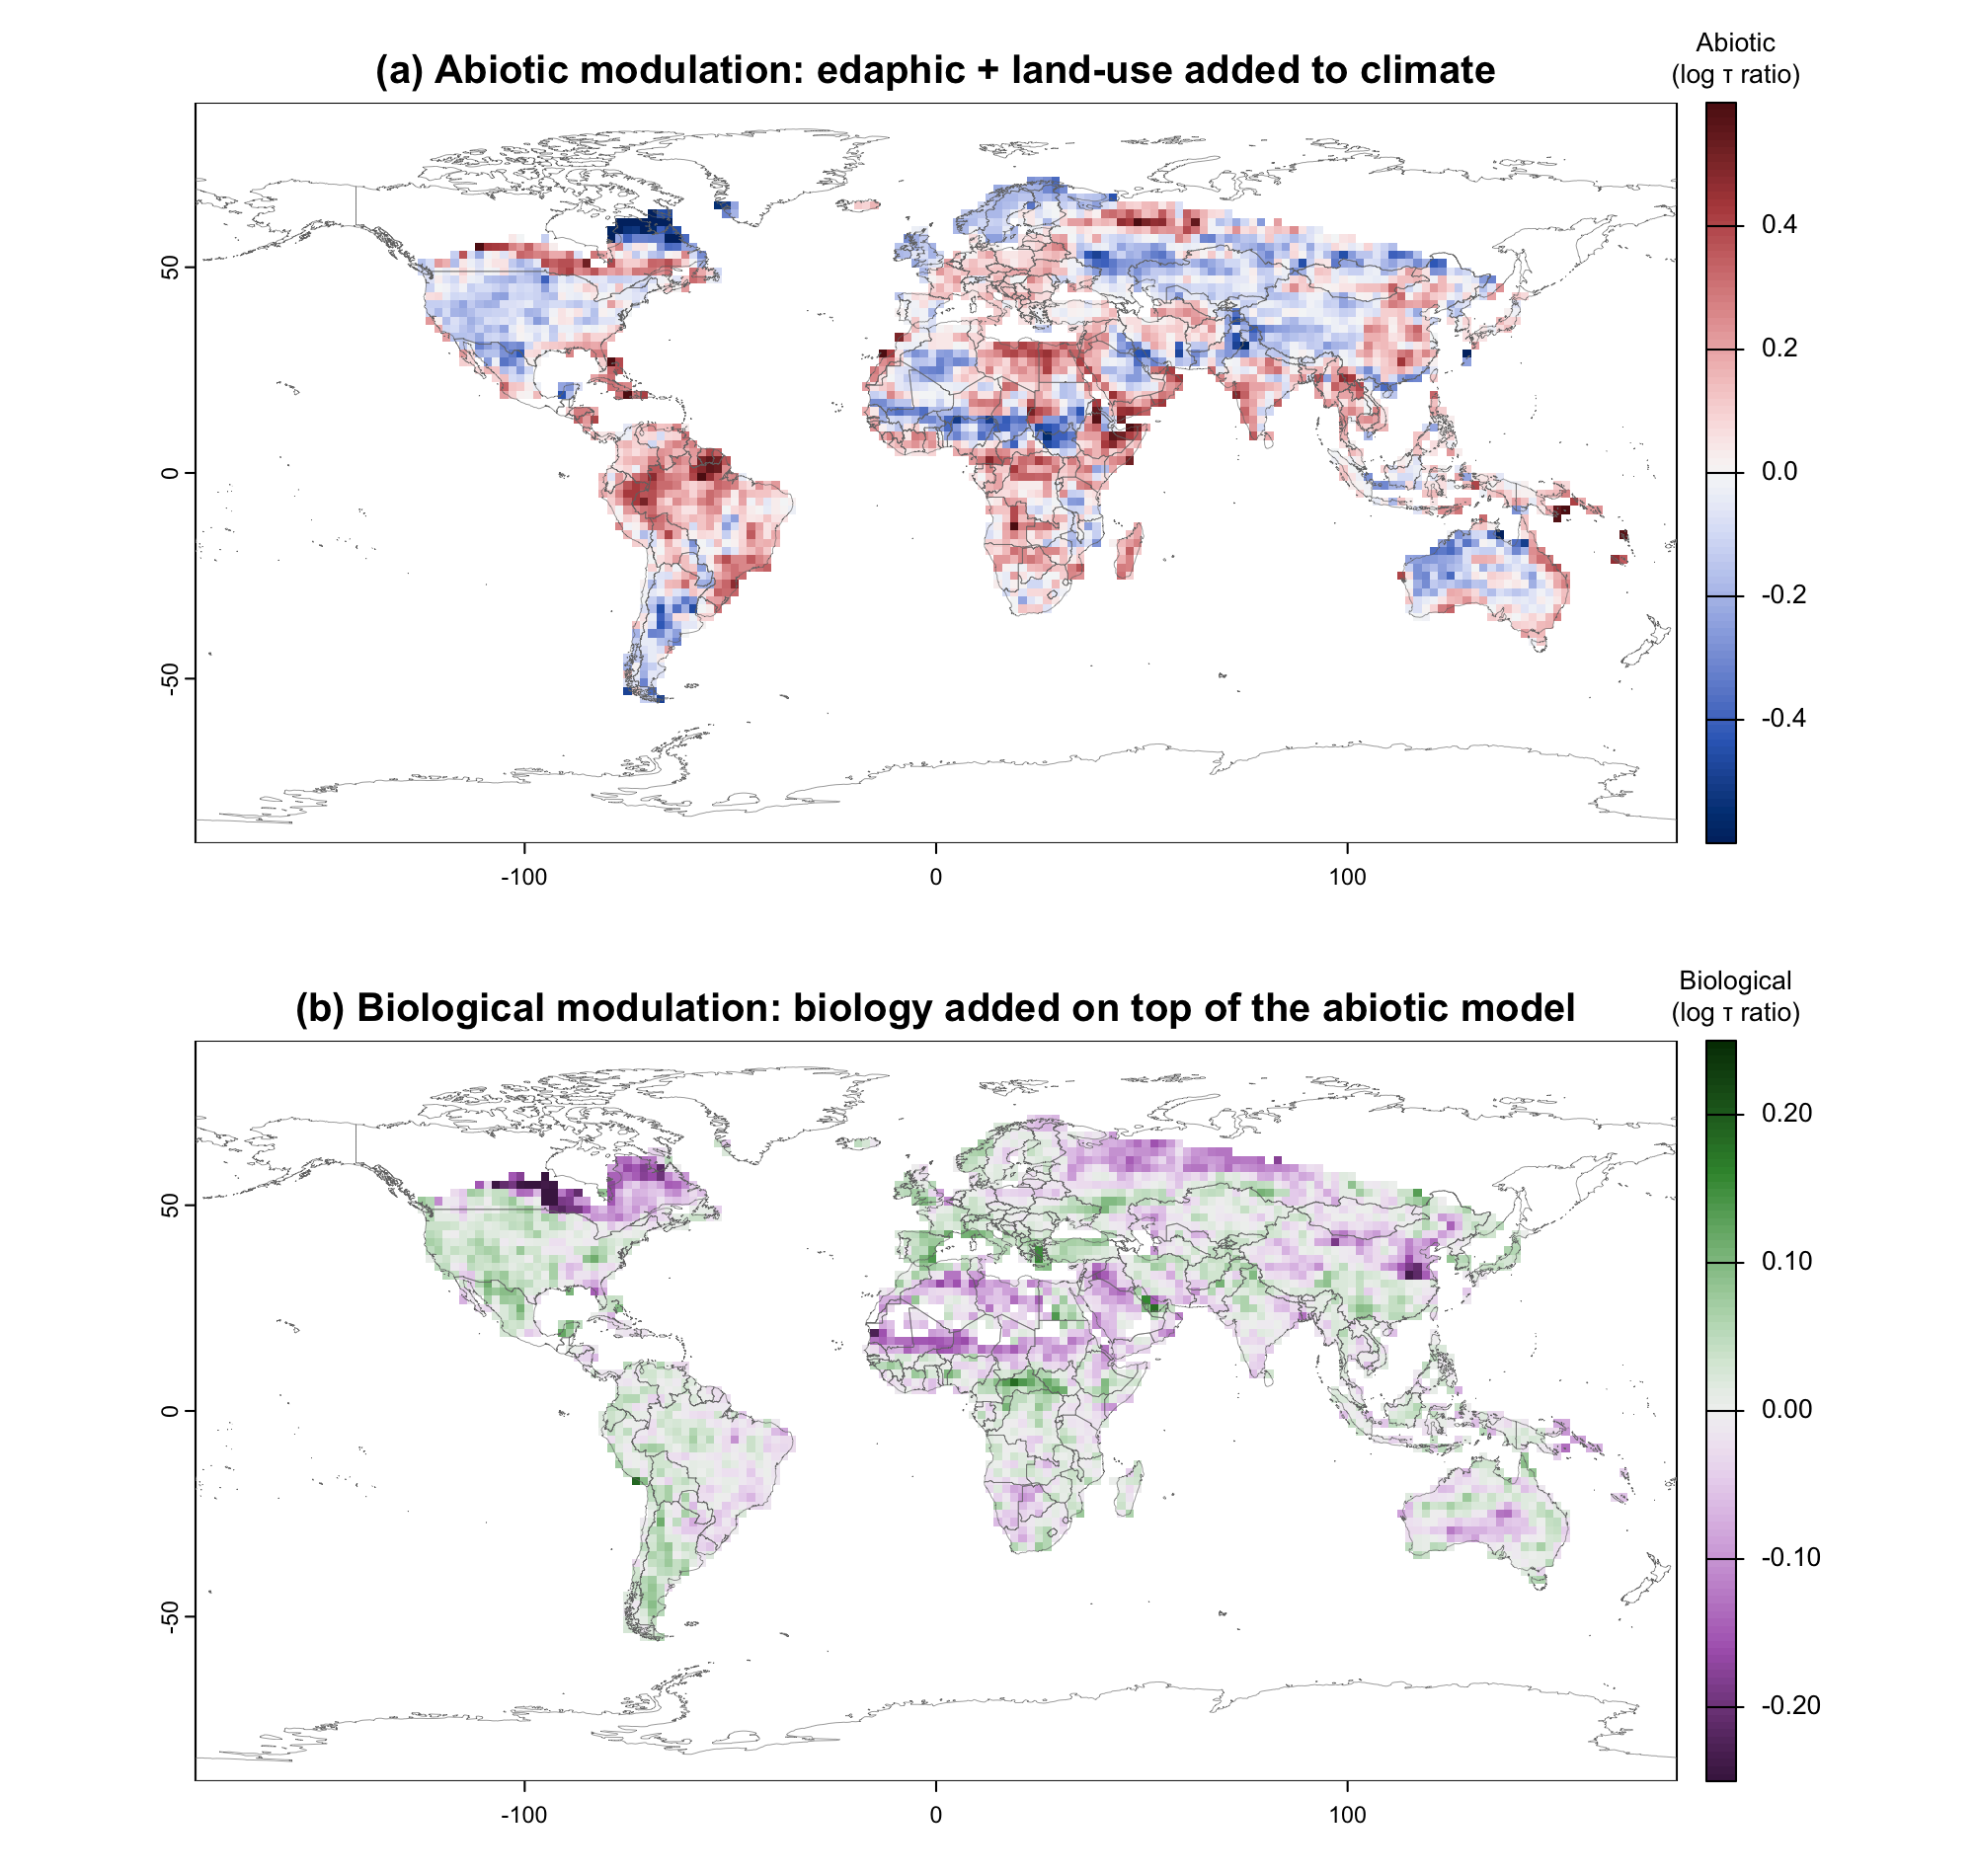
\includegraphics[width=0.80\textwidth]{../../plots/step_15b_zonality/zonality_map_dual.png}
\caption{\textbf{[Appendix] Nested zonality map.} (a) abiotic over climate; (b) biology
\emph{on top of} the abiotic model (order-dependent; biology at its conditional
minimum). Companion to the symmetric main figure. \fpath{15b_zonality_map.R}}
\end{figure}

\begin{figure}[H]\centering
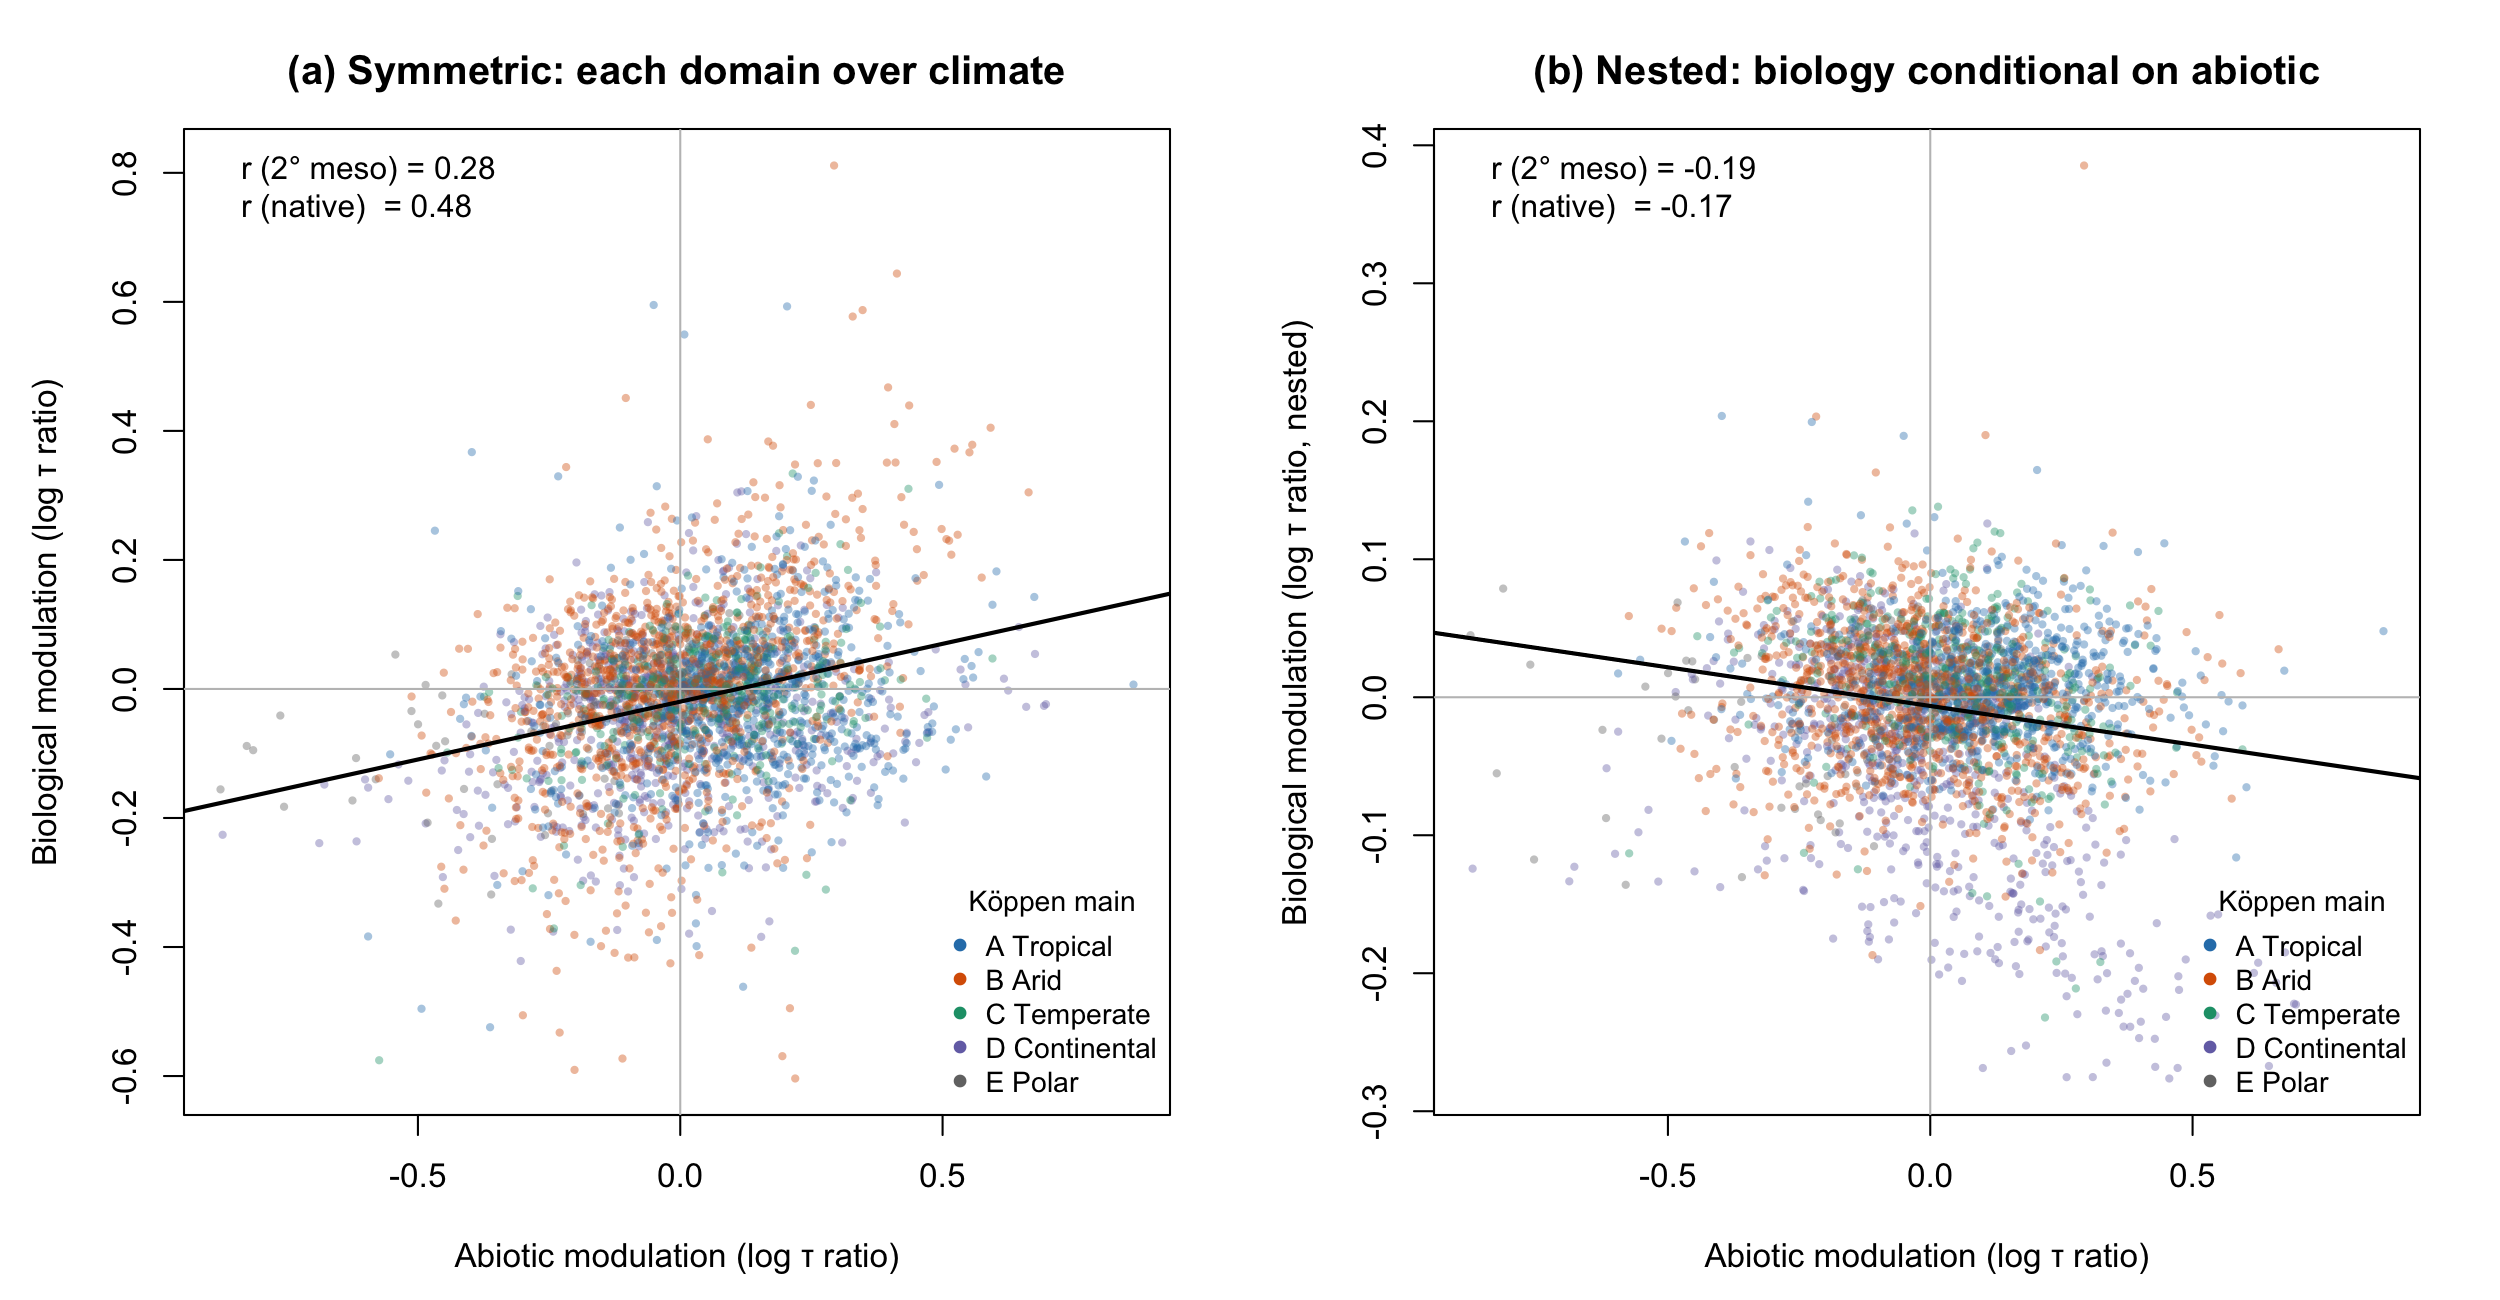
\includegraphics[width=0.72\textwidth]{../../plots/step_15b_zonality/zonality_modulation_scatter.png}
\caption{\textbf{[Appendix] Abiotic vs biological modulation.} K\"oppen-coloured;
symmetric pair co-varies ($r\approx0.4$--$0.5$), nested pair orthogonal
($r\approx0$). ``Correlated, not redundant'' expressed spatially.
\fpath{15b_zonality_map.R}}
\end{figure}

\clearpage
\begin{figure}[H]\centering
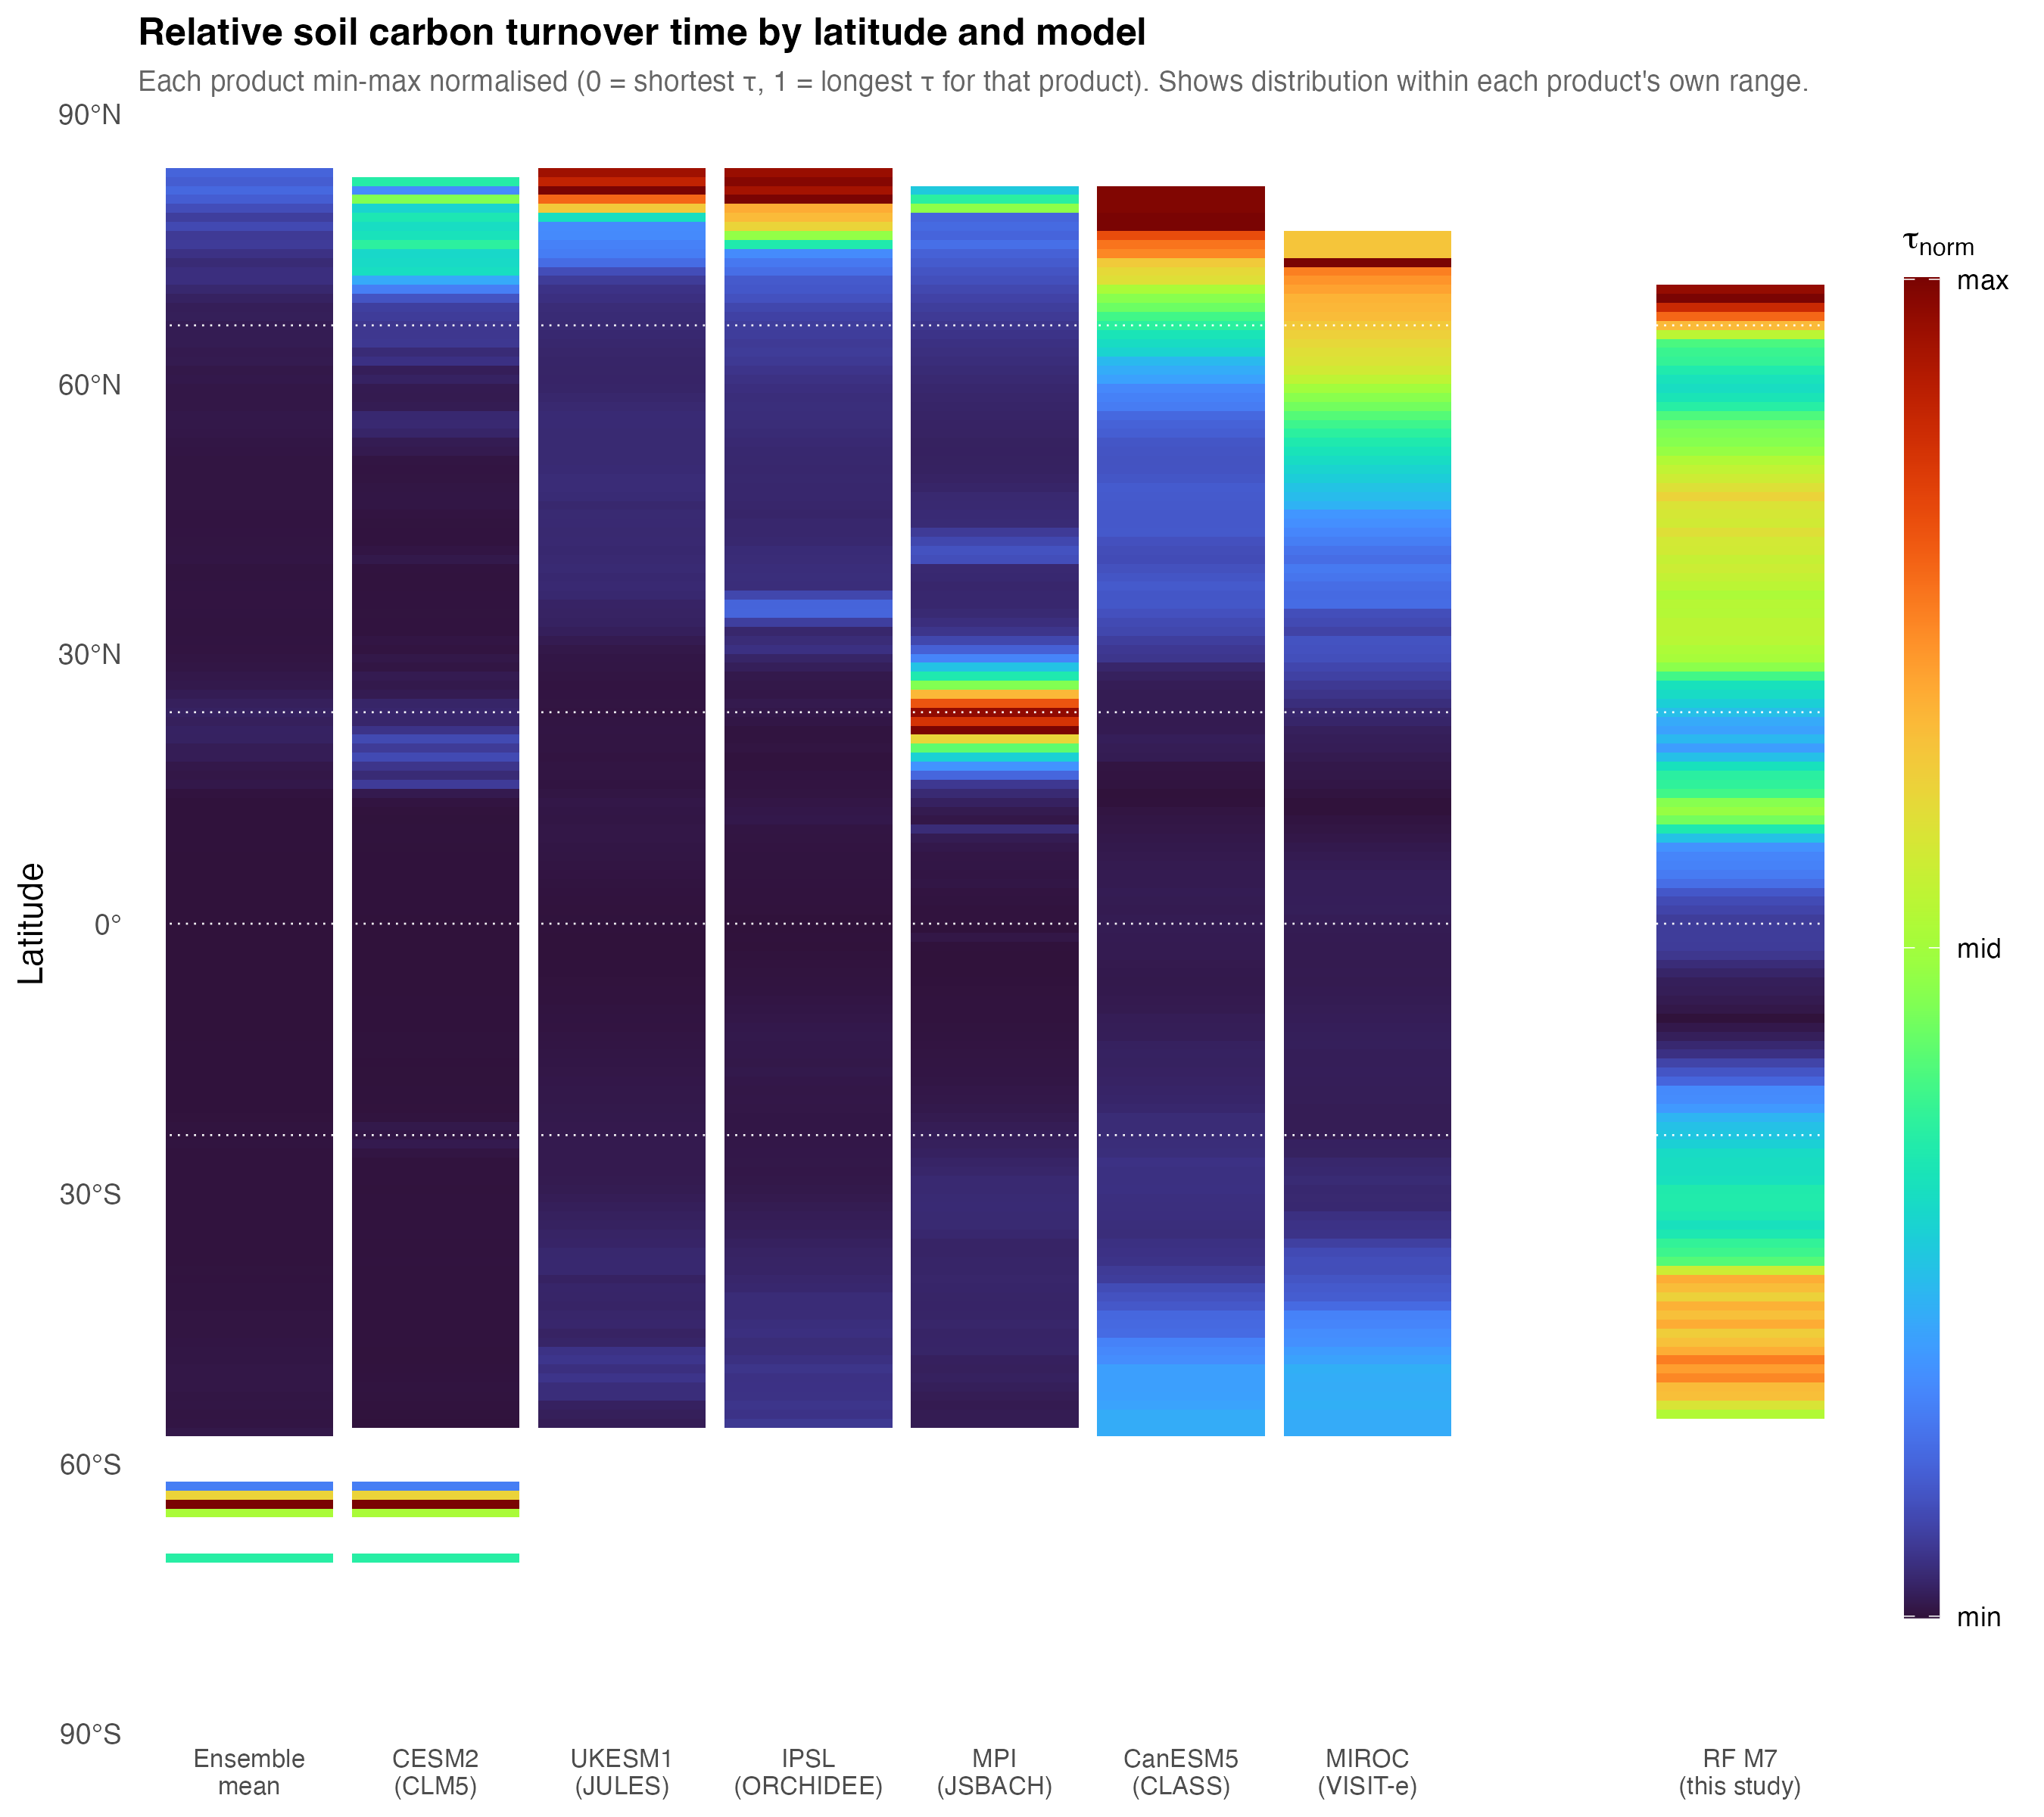
\includegraphics[width=0.92\textwidth]{../../plots/step_20/fig_latitude_heatmap_relative.png}
\caption{\textbf{[SI] Relative latitude heatmap.} Continuous-latitude companion to the
biome-zone ESM figure; each product min--max normalised. \fpath{20_CMIP_comparison.R}}
\end{figure}

\begin{figure}[H]\centering
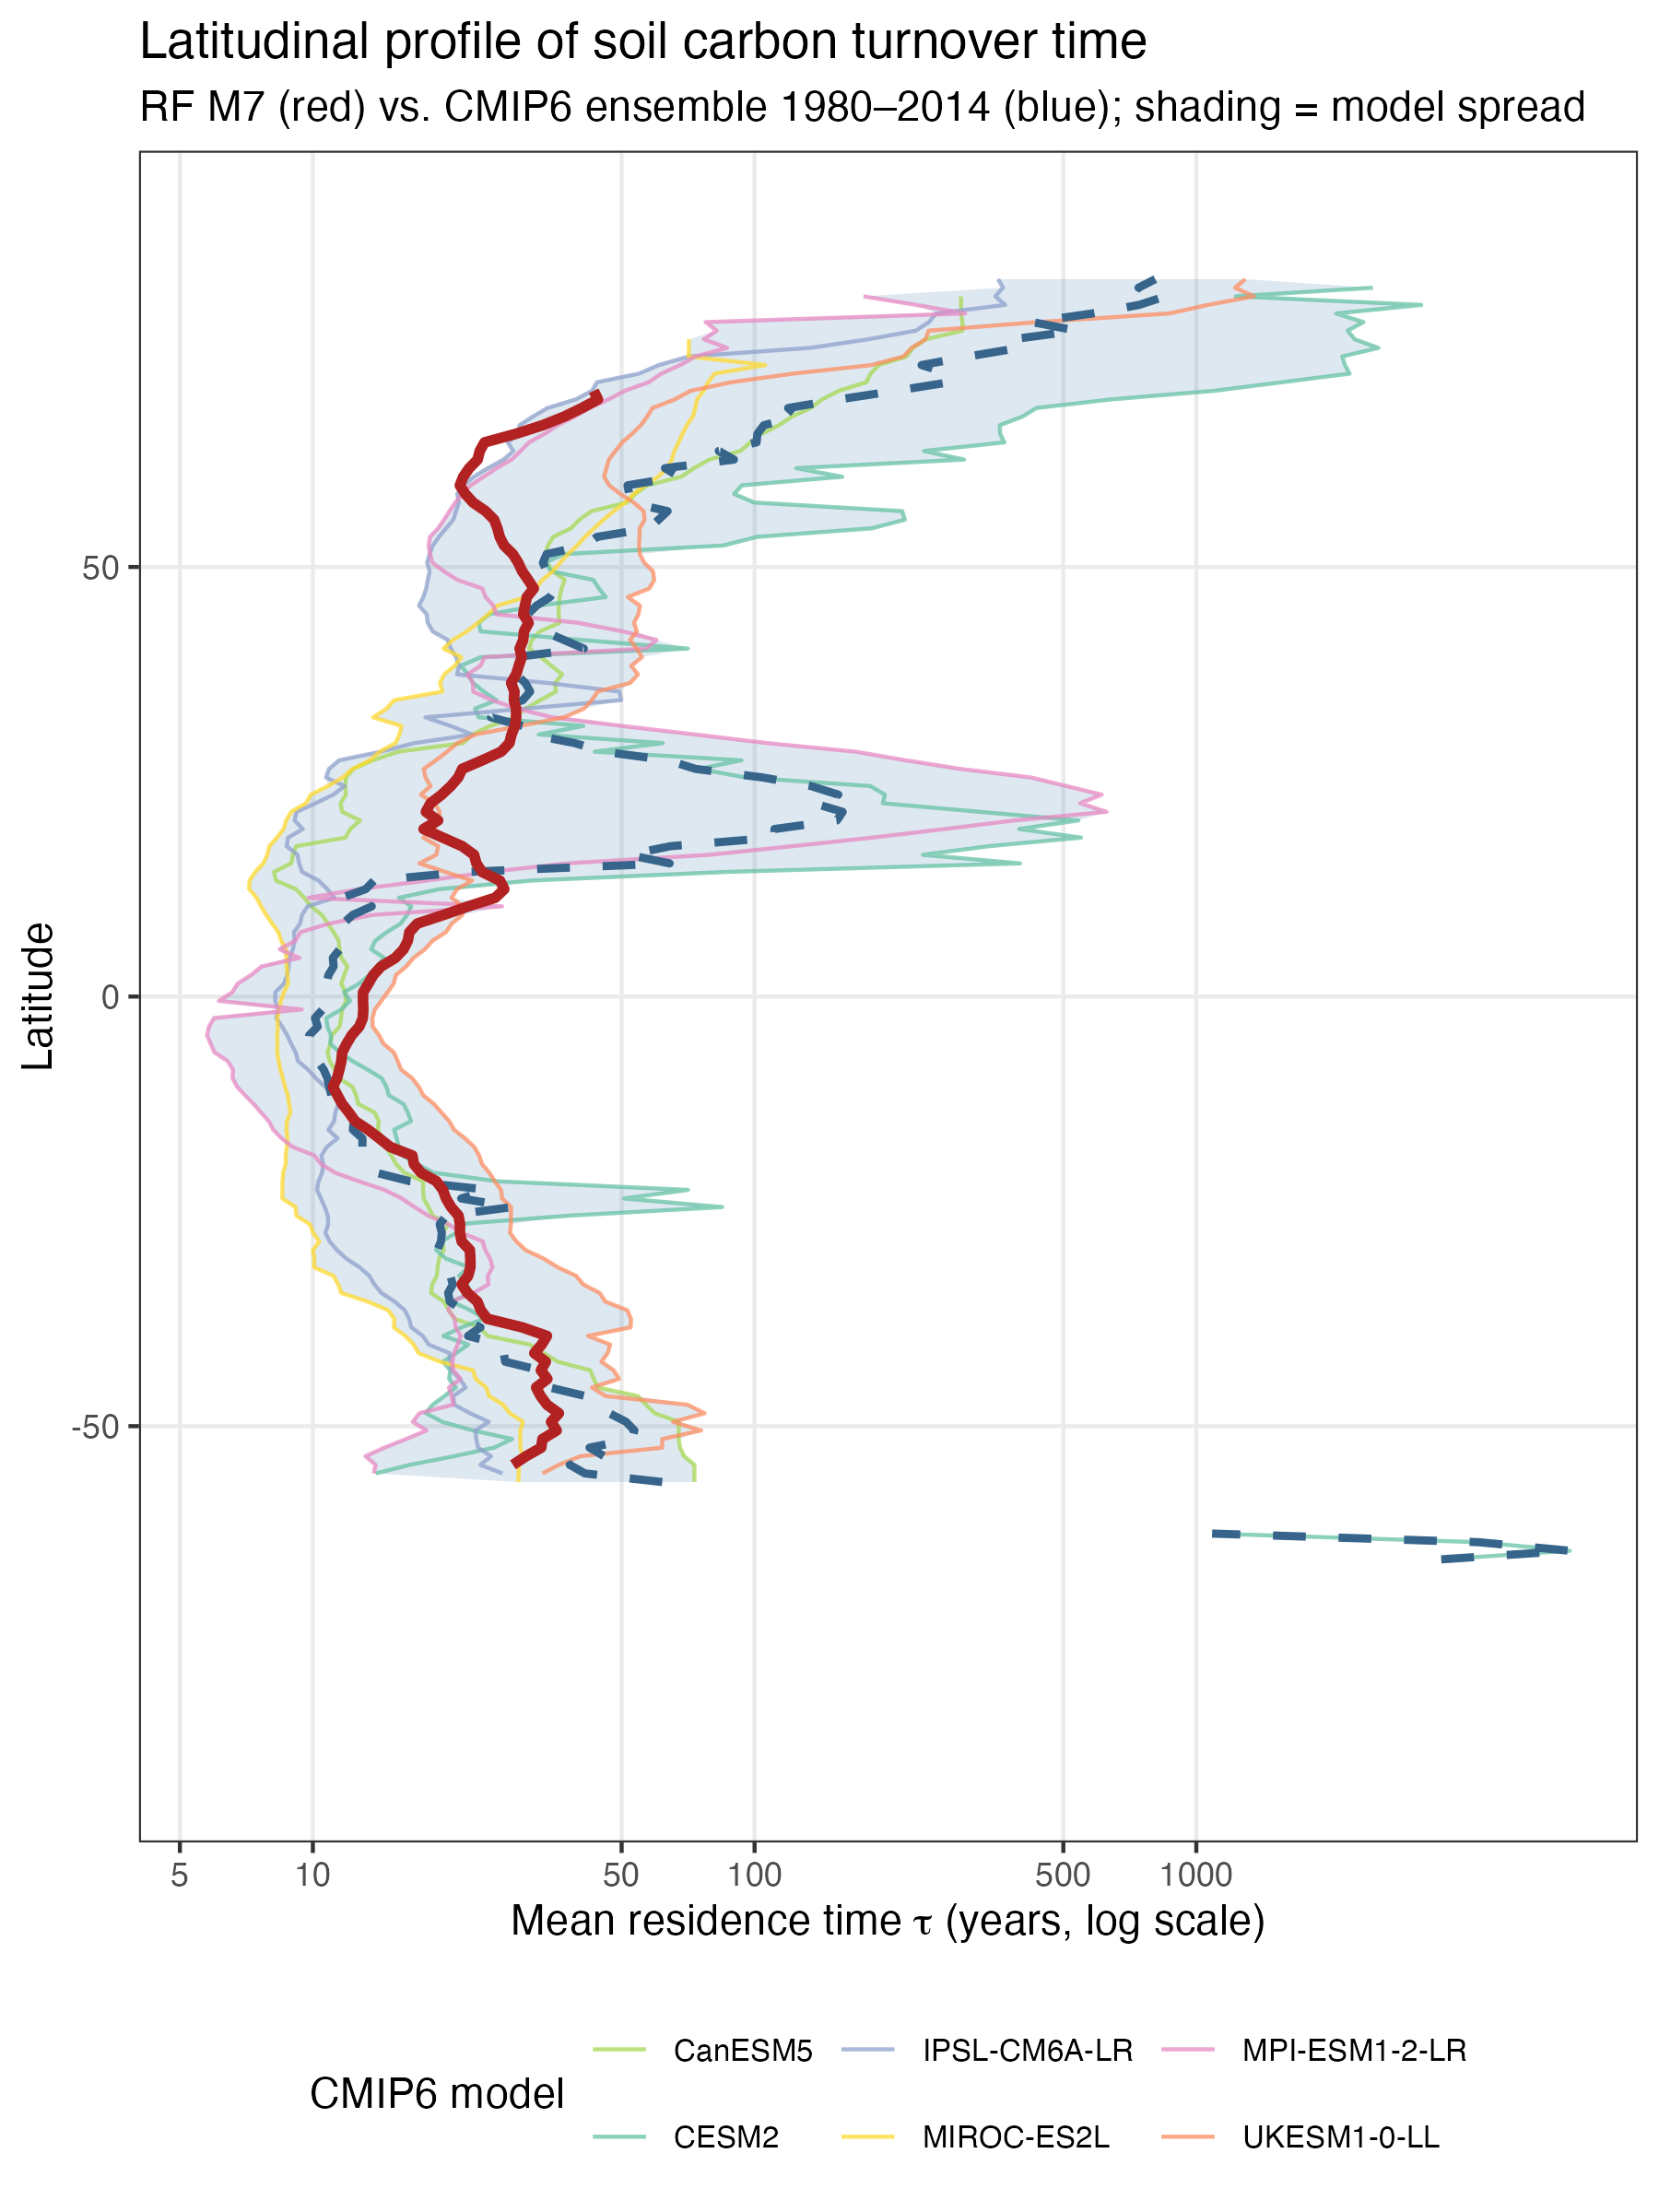
\includegraphics[width=0.85\textwidth]{../../plots/step_20/fig_latitudinal_profile.png}
\caption{\textbf{[Appendix] Absolute latitudinal profile.} The resolved-tension
side-arc: absolute turnover differs across products by depth/pool/reference-period
definitions; shown here, resolved in-text via the normalised structural comparison.
\fpath{20_CMIP_comparison.R}}
\end{figure}

\begin{figure}[H]\centering
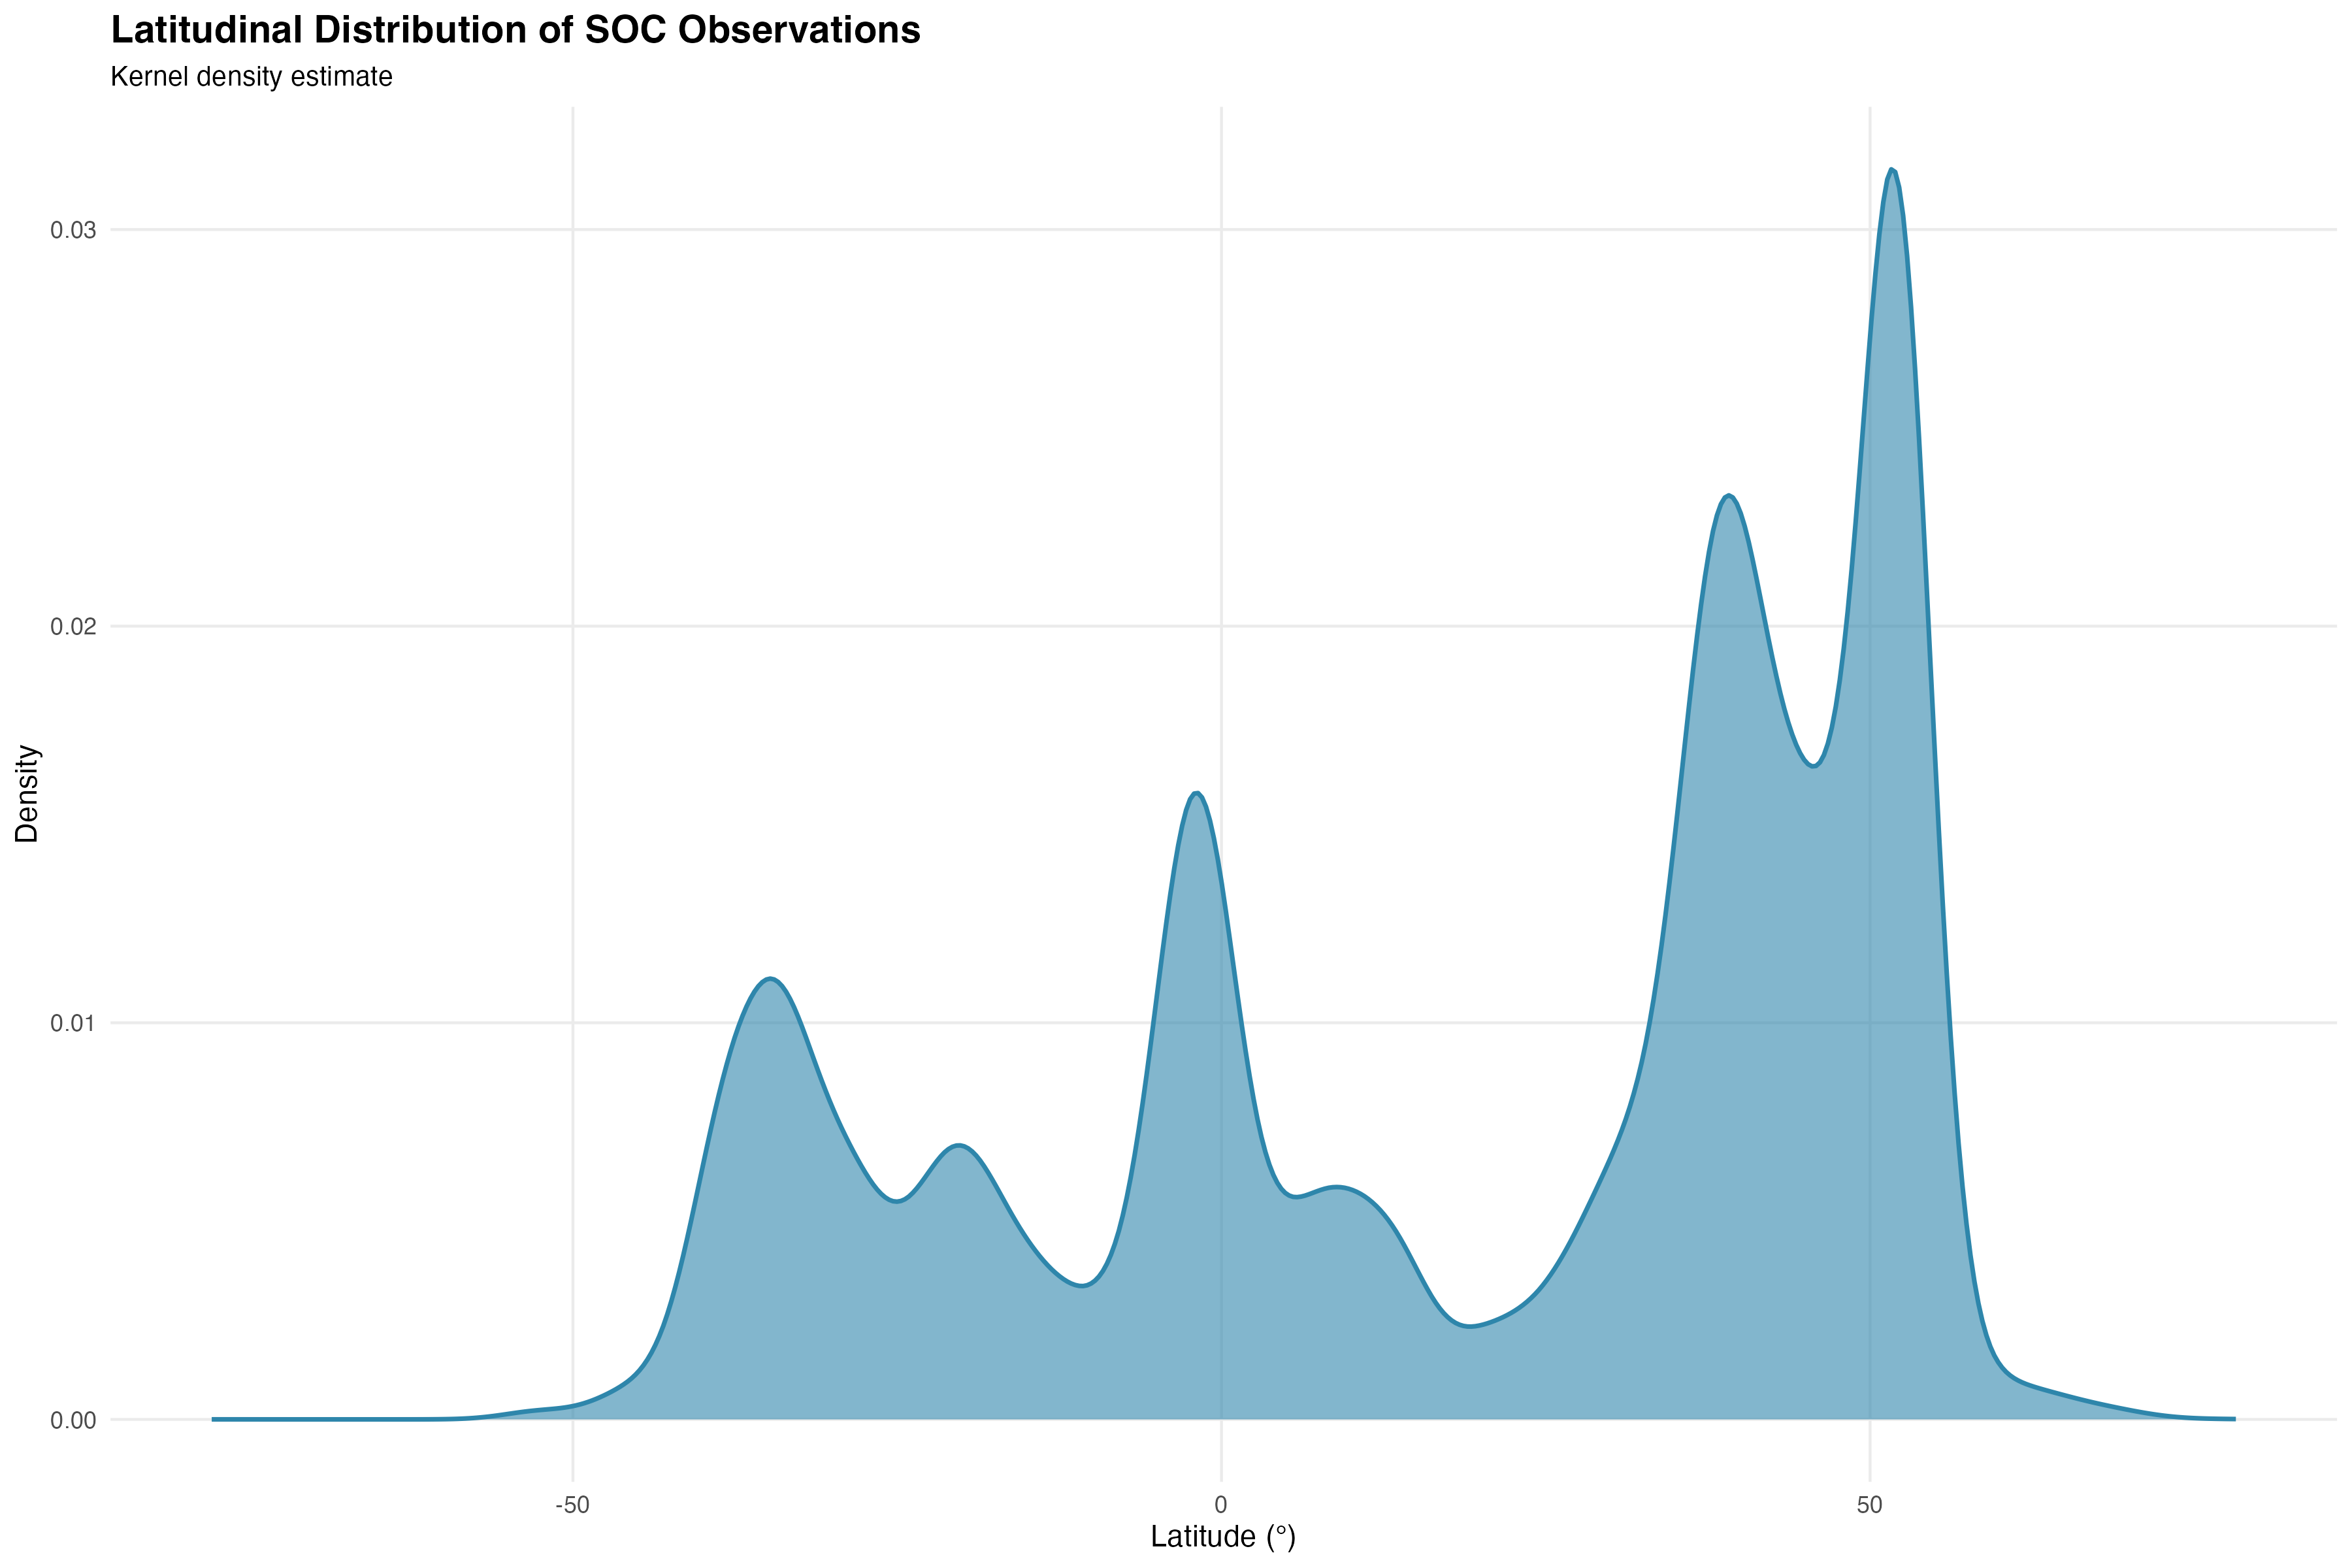
\includegraphics[width=0.85\textwidth]{../../plots/step_17_visualizations/latitudinal_sampling_coverage.png}
\caption{\textbf{[Methods/Data] Latitudinal sampling coverage.} Where and how densely
the OpenLandMap soil profiles sample latitude. \fpath{17_visualizations} (data
description only).}
\end{figure}

\end{document}
